\DocumentMetadata{}
\documentclass[10pt, sigplan]{acmart}
\usepackage[utf8]{inputenc}
\usepackage[T1]{fontenc}

\newcommand{\packageGraphicx}{\usepackage{graphicx}}
\newcommand{\packageHyperref}{\usepackage{hyperref}}
\newcommand{\renewrmdefault}{\renewcommand{\rmdefault}{ptm}}
\newcommand{\packageRelsize}{\usepackage{relsize}}
% amsmath is required for the combination of {mathabx,
% wasysym, newtxmath} to work. Otherwise, newtxmath
% would load amsmath *after* mathabx and wasysym,
% causing command redefinition issues.
\newcommand{\packageAmsmath}{\usepackage{amsmath}}
\newcommand{\packageMathabx}{\usepackage{mathabx}}
% Avoid conflicts between "mathabx" and "wasysym",
% and between "wasysym" integrals and "amsmath" integrals (iint).
\newcommand{\packageWasysym}{
  \let\leftmoon\relax \let\rightmoon\relax \let\fullmoon\relax \let\newmoon\relax \let\diameter\relax
  \usepackage[nointegrals]{wasysym}}
% Both newtxmath and mathabx define the \widering command.
% The only reason we choose the newtxmath version is that
% acmart.cls is also using the one from newtxmath.
\newcommand{\packageTxfonts}{
  \let\widering\relax
  \let\oldwidebar\widebar
  \let\widebar\relax
  \usepackage{newtxmath}
  % if newtxmath is before version 1.7.0,
  % then we are still going to use widebar from mathabx
  \ifx\widebar\relax
    \let\widebar\oldwidebar
  \fi
}
\newcommand{\packageTextcomp}{\usepackage{textcomp}}
\newcommand{\packageFramed}{\usepackage{framed}}
\newcommand{\packageHyphenat}{\usepackage[htt]{hyphenat}}
\newcommand{\packageColor}{\usepackage[usenames,dvipsnames]{color}}
\newcommand{\doHypersetup}{\hypersetup{bookmarks=true,bookmarksopen=true,bookmarksnumbered=true}}
\newcommand{\packageTocstyle}{}
\newcommand{\packageCJK}{\IfFileExists{CJK.sty}{\usepackage{CJK}}{}}
%%%%%%%%%%%%%%%%%%%%%%%%%%%%%%%%%%%%%%%%%%%%%%%%%%%%%%%%%%%%%%%%%%%%%%%%%%%%%%%%
% BEGIN acmart-load.tex
% Avoid package option conflict
\renewcommand\packageColor\relax
\renewcommand\packageTocstyle\relax
\renewcommand\packageMathabx{\ifx\bigtimes\undefined \usepackage{mathabx} \else \relax \fi}
% Both 'mathabx' and 'newtxmath' (required by the 'acmart' class) define a '\bigtimes' command. 
\renewcommand\packageTxfonts\relax
\let\Footnote\undefined
\let\captionwidth\undefined
\renewcommand{\renewrmdefault}{}
% END acmart-load.tex
%%%%%%%%%%%%%%%%%%%%%%%%%%%%%%%%%%%%%%%%%%%%%%%%%%%%%%%%%%%%%%%%%%%%%%%%%%%%%%%%
% This is the default style configuration for Scribble-generated Latex

\packageGraphicx
\packageHyperref
\renewrmdefault
\packageRelsize
\packageAmsmath
\packageMathabx
\packageWasysym
\packageTxfonts
\packageTextcomp
\packageFramed
\packageHyphenat
\packageColor
\doHypersetup
\packageTocstyle
\packageCJK


%%%%%%%%%%%%%%%%%%%%%%%%%%%%%%%%%%%%%%%%%%%%%%%%%%%%%%%%%%%%%%%%%%%%%%%%%%%%%%%%
% Configuration that is especially meant to be overridden:

% Inserted before every ``chapter'', useful for starting each one on a new page:
\newcommand{\sectionNewpage}{}
% Inserted before every book ``part''
\newcommand{\partNewpage}{\sectionNewpage}

% Hooks for actions within the `document' environment:
\newcommand{\preDoc}{}
\newcommand{\postDoc}{}

% Generated by `secref'; first arg is section number, second is section title:
\newcommand{\BookRef}[2]{\emph{#2}}
\newcommand{\ChapRef}[2]{\SecRef{#1}{#2}}
\newcommand{\SecRef}[2]{section~#1}
\newcommand{\PartRef}[2]{part~#1}
% Generated by `Secref':
\newcommand{\BookRefUC}[2]{\BookRef{#1}{#2}}
\newcommand{\ChapRefUC}[2]{\SecRefUC{#1}{#2}}
\newcommand{\SecRefUC}[2]{Section~#1}
\newcommand{\PartRefUC}[2]{Part~#1}

% Variants of the above with a label for an internal reference:
\newcommand{\BookRefLocal}[3]{\hyperref[#1]{\BookRef{#2}{#3}}}
\newcommand{\ChapRefLocal}[3]{\hyperref[#1]{\ChapRef{#2}{#3}}}
\newcommand{\SecRefLocal}[3]{\hyperref[#1]{\SecRef{#2}{#3}}}
\newcommand{\PartRefLocal}[3]{\hyperref[#1]{\PartRef{#2}{#3}}}
\newcommand{\BookRefLocalUC}[3]{\hyperref[#1]{\BookRefUC{#2}{#3}}}
\newcommand{\ChapRefLocalUC}[3]{\hyperref[#1]{\ChapRefUC{#2}{#3}}}
\newcommand{\SecRefLocalUC}[3]{\hyperref[#1]{\SecRefUC{#2}{#3}}}
\newcommand{\PartRefLocalUC}[3]{\hyperref[#1]{\PartRefUC{#2}{#3}}}

% Variants of the above with a section number is empty (i.e., UnNumbered):
\newcommand{\BookRefUN}[1]{\BookRef{}{#1}}
\newcommand{\ChapRefUN}[1]{\SecRefUN{#1}}
\newcommand{\SecRefUN}[1]{``#1''}
\newcommand{\PartRefUN}[1]{\SecRefUN{#1}}
\newcommand{\BookRefUCUN}[1]{\BookRefUN{#1}}
\newcommand{\ChapRefUCUN}[1]{\ChapRefUN{#1}}
\newcommand{\SecRefUCUN}[1]{\SecRefUN{#1}}
\newcommand{\PartRefUCUN}[1]{\PartRefUN{#1}}

\newcommand{\BookRefLocalUN}[2]{\hyperref[#1]{\BookRefUN{#2}}}
\newcommand{\ChapRefLocalUN}[2]{\SecRefLocalUN{#1}{#2}}
\newcommand{\SecRefLocalUN}[2]{\hyperref[#1]{\SecRefUN{#2}}}
\newcommand{\PartRefLocalUN}[2]{\SecRefLocalUN{#1}{#2}}
\newcommand{\BookRefLocalUCUN}[2]{\BookRefLocalUN{#1}{#2}}
\newcommand{\ChapRefLocalUCUN}[2]{\ChapRefLocalUN{#1}{#2}}
\newcommand{\SecRefLocalUCUN}[2]{\SecRefLocalUN{#1}{#2}}
\newcommand{\PartRefLocalUCUN}[2]{\PartRefLocalUN{#1}{#2}}

\newcommand{\SectionNumberLink}[2]{\hyperref[#1]{#2}}

% Enabled with a 'enable-index-merge part style property. This default
% implementation isn't good enough, because the argument is a
% comma-separated sequence of labels:
\newcommand{\Smanypageref}[1]{\pageref{#1}}

%%%%%%%%%%%%%%%%%%%%%%%%%%%%%%%%%%%%%%%%%%%%%%%%%%%%%%%%%%%%%%%%%%%%%%%%%%%%%%%%
% Fonts

% Font commands used by generated text:
\newcommand{\Scribtexttt}[1]{{\texttt{#1}}}
\newcommand{\textsub}[1]{$_{\hbox{\textsmaller{#1}}}$}
\newcommand{\textsuper}[1]{$^{\hbox{\textsmaller{#1}}}$}
\newcommand{\intextcolor}[2]{\textcolor{#1}{#2}}
\newcommand{\intextrgbcolor}[2]{\textcolor[rgb]{#1}{#2}}
\newcommand{\incolorbox}[2]{{\fboxrule=0pt\fboxsep=0pt\protect\colorbox{#1}{#2}}}
\newcommand{\inrgbcolorbox}[2]{{\fboxrule=0pt\fboxsep=0pt\protect\colorbox[rgb]{#1}{#2}}}
\newcommand{\plainlink}[1]{#1}
\newcommand{\techoutside}[1]{#1}
\newcommand{\techinside}[1]{#1}
\newcommand{\badlink}[1]{#1}
\newcommand{\indexlink}[1]{#1}
\newcommand{\noborder}[1]{#1}
\newcommand{\Smaller}[1]{\textsmaller{#1}}
\newcommand{\Larger}[1]{\textlarger{#1}}
\newcommand{\planetName}[1]{PLane\hspace{-0.1ex}T}
\newcommand{\slant}[1]{{\textsl{#1}}}

% Used for <, >, and | in tt mode. For some fonts and installations,
% there seems to be an encoding issue, so pick T1 explicitly:
\newcommand{\Stttextmore}{{\fontencoding{T1}\selectfont>}}
\newcommand{\Stttextless}{{\fontencoding{T1}\selectfont<}}
\newcommand{\Stttextbar}{{\fontencoding{T1}\selectfont|}}

%%%%%%%%%%%%%%%%%%%%%%%%%%%%%%%%%%%%%%%%%%%%%%%%%%%%%%%%%%%%%%%%%%%%%%%%%%%%%%%%
% Tables

% The `stabular' environment seems to be the lesser of evils among 
%  page-breaking table environments (and we've made a copy as ``pltstabular'
%  to make sure that it doesn't change).

\makeatletter
%%%%%%%%%%%%%%%%%%%%%%%%%%%%%%%%%%%%%%%%%%%%%%%%%%%%%%%%%%%%%%%%%%%%%%
\message{pltstabular is a modification of stabular}
%% A renamed version of:
%% stabular.sty
%% Copyright 1998 Sigitas Tolu\v sis
%% VTeX Ltd., Akademijos 4, Vilnius, Lithuania
%% e-mail sigitas@vtex.lt
%% http://www.vtex.lt/tex/download/macros/
%%
% This program can redistributed and/or modified under the terms
% of the LaTeX Project Public License Distributed from CTAN
% archives in directory macros/latex/base/lppl.txt; either
% version 1 of the License, or (at your option) any later version.
%
% PURPOSE:   Improve tabular environment.
%
% SHORT DESCRIPTION:
%
% Changed internal commands: \@mkpream, \@addamp, \@xhline
%
% Provides new commands in tabular (used after command \\):
% \emptyrow[#1] 
% -------------
%    Adds empty row, #1 - height of the row 
%
% \tabrow{#1}[#2] 
% ---------------
%    Adds row of natural height: #1\\[#2]
%
% Provides new environments: pltstabular and pltstabular* 
%                            --------     ---------
%            One more multi-page version of tabular
%
%
\def\empty@finalstrut#1{%
  \unskip\ifhmode\nobreak\fi\vrule\@width\z@\@height\z@\@depth\z@}
\def\no@strut{\global\setbox\@arstrutbox\hbox{%
    \vrule \@height\z@
           \@depth\z@
           \@width\z@}%
    \gdef\@endpbox{\empty@finalstrut\@arstrutbox\par\egroup\hfil}%
}%
\def\yes@strut{\global\setbox\@arstrutbox\hbox{%
    \vrule \@height\arraystretch \ht\strutbox
           \@depth\arraystretch \dp\strutbox
           \@width\z@}%
    \gdef\@endpbox{\@finalstrut\@arstrutbox\par\egroup\hfil}%
}%
\def\@mkpream#1{\@firstamptrue\@lastchclass6
  \let\@preamble\@empty\def\empty@preamble{\add@ins}%
  \let\protect\@unexpandable@protect
  \let\@sharp\relax\let\add@ins\relax
  \let\@startpbox\relax\let\@endpbox\relax
  \@expast{#1}%
  \expandafter\@tfor \expandafter
    \@nextchar \expandafter:\expandafter=\reserved@a\do
       {\@testpach\@nextchar
    \ifcase \@chclass \@classz \or \@classi \or \@classii \or \@classiii
      \or \@classiv \or\@classv \fi\@lastchclass\@chclass}%
  \ifcase \@lastchclass \@acol
      \or \or \@preamerr \@ne\or \@preamerr \tw@\or \or \@acol \fi}
\def\@addamp{%
  \if@firstamp
    \@firstampfalse
    \edef\empty@preamble{\add@ins}%
  \else
    \edef\@preamble{\@preamble &}%
    \edef\empty@preamble{\expandafter\noexpand\empty@preamble &\add@ins}%
  \fi}
\newif\iftw@hlines \tw@hlinesfalse
\def\@xhline{\ifx\reserved@a\hline
               \tw@hlinestrue
             \else\ifx\reserved@a\Hline
               \tw@hlinestrue
             \else
               \tw@hlinesfalse
             \fi\fi
      \iftw@hlines
        \aftergroup\do@after
      \fi
      \ifnum0=`{\fi}%
}
\def\do@after{\emptyrow[\the\doublerulesep]}
\def\emptyrow{\noalign\bgroup\@ifnextchar[\@emptyrow{\@emptyrow[\z@]}}
\def\@emptyrow[#1]{\no@strut\gdef\add@ins{\vrule \@height\z@ \@depth#1 \@width\z@}\egroup%
\empty@preamble\\
\noalign{\yes@strut\gdef\add@ins{\vrule \@height\z@ \@depth\z@ \@width\z@}}%
}
\def\tabrow#1{\noalign\bgroup\@ifnextchar[{\@tabrow{#1}}{\@tabrow{#1}[]}}
\def\@tabrow#1[#2]{\no@strut\egroup#1\ifx.#2.\\\else\\[#2]\fi\noalign{\yes@strut}}
%
\def\endpltstabular{\crcr\egroup\egroup \egroup}
\expandafter \let \csname endpltstabular*\endcsname = \endpltstabular
\def\pltstabular{\let\@halignto\@empty\@pltstabular}
\@namedef{pltstabular*}#1{\def\@halignto{to#1}\@pltstabular}
\def\@pltstabular{\leavevmode \bgroup \let\@acol\@tabacol
   \let\@classz\@tabclassz
   \let\@classiv\@tabclassiv \let\\\@tabularcr\@stabarray}
\def\@stabarray{\m@th\@ifnextchar[\@sarray{\@sarray[c]}}
\def\@sarray[#1]#2{%
  \bgroup
  \setbox\@arstrutbox\hbox{%
    \vrule \@height\arraystretch\ht\strutbox
           \@depth\arraystretch \dp\strutbox
           \@width\z@}%
  \@mkpream{#2}%
  \edef\@preamble{%
    \ialign \noexpand\@halignto
      \bgroup \@arstrut \@preamble \tabskip\z@skip \cr}%
  \let\@startpbox\@@startpbox \let\@endpbox\@@endpbox
  \let\tabularnewline\\%
%    \let\par\@empty
    \let\@sharp##%
    \set@typeset@protect
    \lineskip\z@skip\baselineskip\z@skip
    \@preamble}

%%%%%%%%%%%%%%%%%%%%%%%%%%%%%%%%%%%%%%%%%%%%%%%%%%%%%%%%%%%%%%%%%%%%%%
\makeatother

\newenvironment{bigtabular}{\begin{pltstabular}}{\end{pltstabular}}
% For the 'boxed table style:
\newcommand{\SBoxedLeft}{\textcolor[rgb]{0.6,0.6,1.0}{\vrule width 3pt\hspace{3pt}}}
% Formerly used to keep the horizontal line for a definition on the same page:
\newcommand{\SEndFirstHead}[0]{ \nopagebreak \\ }
% Corrects weirdness when a table is the first thing in
%  an itemization:
\newcommand{\bigtableinlinecorrect}[0]{~

\vspace{-\baselineskip}\vspace{\parskip}}
% Used to indent the table correctly in an itemization, since that's
%  one of the things stabular gets wrong:
\newlength{\stabLeft}
\newcommand{\bigtableleftpad}{\hspace{\stabLeft}}
\newcommand{\atItemizeStart}[0]{\addtolength{\stabLeft}{\labelsep}
                                \addtolength{\stabLeft}{\labelwidth}}


% For a single-column table in simple environments, it's better to
%  use the `list' environment instead of `stabular'.
\newenvironment{SingleColumn}{\begin{list}{}{\topsep=0pt\partopsep=0pt%
\listparindent=0pt\itemindent=0pt\labelwidth=0pt\leftmargin=0pt\rightmargin=0pt%
\itemsep=0pt\parsep=0pt}\item}{\end{list}}

%%%%%%%%%%%%%%%%%%%%%%%%%%%%%%%%%%%%%%%%%%%%%%%%%%%%%%%%%%%%%%%%%%%%%%%%%%%%%%%%
% Etc.

% ._ and .__
\newcommand{\Sendabbrev}[1]{#1\@}
\newcommand{\Sendsentence}[1]{\@#1}

% Default style for a nested flow:
\newenvironment{Subflow}{\begin{list}{}{\topsep=0pt\partopsep=0pt%
\listparindent=0pt\itemindent=0pt\labelwidth=0pt\leftmargin=0pt\rightmargin=0pt%
\itemsep=0pt}\item}{\end{list}}

% For the 'inset nested-flow style:
\newenvironment{SInsetFlow}{\begin{quote}}{\end{quote}}

% Indent a 'code-inset nested flow:
\newcommand{\SCodePreSkip}{\vskip\abovedisplayskip}
\newcommand{\SCodePostSkip}{\vskip\belowdisplayskip}
\newenvironment{SCodeFlow}{\SCodePreSkip\begin{list}{}{\topsep=0pt\partopsep=0pt%
\listparindent=0pt\itemindent=0pt\labelwidth=0pt\leftmargin=2ex\rightmargin=2ex%
\itemsep=0pt\parsep=0pt}\item}{\end{list}\SCodePostSkip}
\newcommand{\SCodeInsetBox}[1]{\setbox1=\hbox{\hbox{\hspace{2ex}#1\hspace{2ex}}}\vbox{\SCodePreSkip\vtop{\box1\SCodePostSkip}}}

% Inset a 'vertical-inset nested flow:
\newcommand{\SVInsetPreSkip}{\vskip\abovedisplayskip}
\newcommand{\SVInsetPostSkip}{\vskip\belowdisplayskip}
\newenvironment{SVInsetFlow}{\SVInsetPreSkip\begin{list}{}{\topsep=0pt\partopsep=0pt%
\listparindent=0pt\itemindent=0pt\labelwidth=0pt\leftmargin=0pt\rightmargin=0pt%
\itemsep=0pt\parsep=0pt}\item}{\end{list}\SVInsetPostSkip}
\newcommand{\SVInsetBox}[1]{\setbox1=\hbox{\hbox{#1}}\vbox{\SCodePreSkip\vtop{\box1\SCodePostSkip}}}

% The 'compact itemization style:
\newenvironment{compact}{\begin{itemize}}{\end{itemize}}
\newcommand{\compactItem}[1]{\item #1}

% The nested-flow style for `centerline':
\newenvironment{SCentered}{\begin{trivlist}\item \centering}{\end{trivlist}}

% The \refpara command corresponds to `margin-note'. The
% refcolumn and refcontent environments also wrap the note,
% because they simplify the CSS side.
\newcommand{\refpara}[1]{\normalmarginpar\marginpar{\raggedright \footnotesize #1}}
\newcommand{\refelem}[1]{\refpara{#1}}
\newenvironment{refcolumn}{}{}
\newenvironment{refcontent}{}{}

\newcommand{\refparaleft}[1]{\reversemarginpar\marginpar{\raggedright \footnotesize #1}}
\newcommand{\refelemleft}[1]{\refparaleft{#1}}
\newenvironment{refcolumnleft}{}{}

% Macros used by `title' and `author':
\newcommand{\titleAndVersionAndAuthors}[3]{\title{#1\\{\normalsize \SVersionBefore{}#2}}\author{#3}\maketitle}
\newcommand{\titleAndVersionAndEmptyAuthors}[3]{\title{#1\\{\normalsize \SVersionBefore{}#2}}#3\maketitle}
\newcommand{\titleAndEmptyVersionAndAuthors}[3]{\title{#1}\author{#3}\maketitle}
\newcommand{\titleAndEmptyVersionAndEmptyAuthors}[3]{\title{#1}\maketitle}
\newcommand{\titleAndVersionAndAuthorsAndShort}[4]{\title[#4]{#1\\{\normalsize \SVersionBefore{}#2}}\author{#3}\maketitle}
\newcommand{\titleAndVersionAndEmptyAuthorsAndShort}[4]{\title[#4]{#1\\{\normalsize \SVersionBefore{}#2}}#3\maketitle}
\newcommand{\titleAndEmptyVersionAndAuthorsAndShort}[4]{\title[#4]{#1}\author{#3}\maketitle}
\newcommand{\titleAndEmptyVersionAndEmptyAuthorsAndShort}[4]{\title[#4]{#1}\maketitle}
\newcommand{\SAuthor}[1]{#1}
\newcommand{\SAuthorSep}[1]{\qquad}
\newcommand{\SVersionBefore}[1]{Version }

% Useful for some styles, such as sigalternate:
\newcommand{\SNumberOfAuthors}[1]{}

\let\SOriginalthesubsection\thesubsection
\let\SOriginalthesubsubsection\thesubsubsection

% sections
\newcommand{\Spart}[2]{\part[#1]{#2}}
\newcommand{\Ssection}[2]{\section[#1]{#2}\let\thesubsection\SOriginalthesubsection}
\newcommand{\Ssubsection}[2]{\subsection[#1]{#2}\let\thesubsubsection\SOriginalthesubsubsection}
\newcommand{\Ssubsubsection}[2]{\subsubsection[#1]{#2}}
\newcommand{\Ssubsubsubsection}[2]{{\bf #2}}
\newcommand{\Ssubsubsubsubsection}[2]{\Ssubsubsubsection{#1}{#2}}

% "star" means unnumbered and not in ToC:
\newcommand{\Spartstar}[1]{\part*{#1}}
\newcommand{\Ssectionstar}[1]{\section*{#1}\renewcommand*\thesubsection{\arabic{subsection}}\setcounter{subsection}{0}}
\newcommand{\Ssubsectionstar}[1]{\subsection*{#1}\renewcommand*\thesubsubsection{\arabic{section}.\arabic{subsubsection}}\setcounter{subsubsection}{0}}
\newcommand{\Ssubsubsectionstar}[1]{\subsubsection*{#1}}
\newcommand{\Ssubsubsubsectionstar}[1]{{\bf #1}}
\newcommand{\Ssubsubsubsubsectionstar}[1]{\Ssubsubsubsectionstar{#1}}

% "starx" means unnumbered but in ToC:
\newcommand{\Spartstarx}[2]{\Spartstar{#2}\phantomsection\addcontentsline{toc}{part}{#1}}
\newcommand{\Ssectionstarx}[2]{\Ssectionstar{#2}\phantomsection\addcontentsline{toc}{section}{#1}}
\newcommand{\Ssubsectionstarx}[2]{\Ssubsectionstar{#2}\phantomsection\addcontentsline{toc}{subsection}{#1}}
\newcommand{\Ssubsubsectionstarx}[2]{\Ssubsubsectionstar{#2}\phantomsection\addcontentsline{toc}{subsubsection}{#1}}
\newcommand{\Ssubsubsubsectionstarx}[2]{\Ssubsubsubsectionstar{#2}}
\newcommand{\Ssubsubsubsubsectionstarx}[2]{\Ssubsubsubsubsectionstar{#2}}

% "grouper" is for the 'grouper style variant --- on subsections and lower,
%  because \Spart is used for grouper at the section level. Grouper implies
%  unnumbered.
\newcounter{GrouperTemp}
\newcommand{\Ssubsectiongrouper}[2]{\setcounter{GrouperTemp}{\value{subsection}}\Ssubsectionstarx{#1}{#2}\setcounter{subsection}{\value{GrouperTemp}}}
\newcommand{\Ssubsubsectiongrouper}[2]{\setcounter{GrouperTemp}{\value{subsubsection}}\Ssubsubsectionstarx{#1}{#2}\setcounter{subsubsection}{\value{GrouperTemp}}}
\newcommand{\Ssubsubsubsectiongrouper}[2]{\Ssubsubsubsectionstarx{#1}{#2}}
\newcommand{\Ssubsubsubsubsectiongrouper}[2]{\Ssubsubsubsubsectionstarx{#1}{#2}}

\newcommand{\Ssubsectiongrouperstar}[1]{\setcounter{GrouperTemp}{\value{subsection}}\Ssubsectionstar{#1}\setcounter{subsection}{\value{GrouperTemp}}}
\newcommand{\Ssubsubsectiongrouperstar}[1]{\setcounter{GrouperTemp}{\value{subsubsection}}\Ssubsubsectionstar{#1}\setcounter{subsubsection}{\value{GrouperTemp}}}
\newcommand{\Ssubsubsubsectiongrouperstar}[1]{\Ssubsubsubsectionstar{#1}}
\newcommand{\Ssubsubsubsubsectiongrouperstar}[1]{\Ssubsubsubsubsectionstar{#1}}

\newcommand{\Ssubsectiongrouperstarx}[2]{\setcounter{GrouperTemp}{\value{subsection}}\Ssubsectionstarx{#1}{#2}\setcounter{subsection}{\value{GrouperTemp}}}
\newcommand{\Ssubsubsectiongrouperstarx}[2]{\setcounter{GrouperTemp}{\value{subsubsection}}\Ssubsubsectionstarx{#1}{#2}\setcounter{subsubsection}{\value{GrouperTemp}}}
\newcommand{\Ssubsubsubsectiongrouperstarx}[2]{\Ssubsubsubsectionstarx{#1}{#2}}
\newcommand{\Ssubsubsubsubsectiongrouperstarx}[2]{\Ssubsubsubsubsectionstarx{#1}{#2}}

% Generated by `subsubsub*section':
\newcommand{\SSubSubSubSection}[1]{\Ssubsubsubsubsectionstar{#1}}

% For hidden parts with an empty title:
\newcommand{\notitlesection}{\vspace{2ex}\phantomsection\noindent}

% To increment section numbers:
\newcommand{\Sincpart}{\stepcounter{part}}
\newcommand{\Sincsection}{\stepcounter{section}}
\newcommand{\Sincsubsection}{\stepcounter{subsection}}
\newcommand{\Sincsubsubsection}{\stepcounter{subsubsection}}
\newcommand{\Sincsubsubsubsection}{}
\newcommand{\Sincsubsubsubsubsection}{}

% When brackets appear in section titles:
\newcommand{\SOpenSq}{[}
\newcommand{\SCloseSq}{]}

% Helper for box-mode macros:
\newcommand{\Svcenter}[1]{$\vcenter{#1}$}

% Verbatim
\newenvironment{SVerbatim}{}{}

% Helper to work around a problem with "#"s for URLs within \href
% within other macros:
\newcommand{\Shref}[3]{\href{#1\##2}{#3}}

% For URLs:
\newcommand{\Snolinkurl}[1]{\nolinkurl{#1}}

% History note:
\newcommand{\SHistory}[1]{\begin{smaller}#1\end{smaller}}

%%%%%%%%%%%%%%%%%%%%%%%%%%%%%%%%%%%%%%%%%%%%%%%%%%%%%%%%%%%%%%%%%%%%%%%%%%%%%%%%

% Scribble then generates the following:
%
%  \begin{document}
%  \preDoc
%  \titleAndVersion{...}{...}
%  ... document content ...
%  \postDoc
%  \end{document}
%%%%%%%%%%%%%%%%%%%%%%%%%%%%%%%%%%%%%%%%%%%%%%%%%%%%%%%%%%%%%%%%%%%%%%%%%%%%%%%%
% BEGIN acmart/acmart.tex
% Support for styles in scribble/acmart

% These are replaced by scribble/acmart/style.tex,
%  which is used in combination with acmart.cls

\newcommand{\SAuthorinfo}[4]{#1}
\newcommand{\SAuthorPlace}[1]{#1}
\newcommand{\SAuthorEmail}[1]{#1}
\newcommand{\SAuthorOrcid}[1]{#1}

\newcommand{\SConferenceInfo}[2]{}
\newcommand{\SCopyrightYear}[1]{}
\newcommand{\SCopyrightData}[1]{}
\newcommand{\Sdoi}[1]{}
\newcommand{\SPexclusivelicense}[0]{}

\newcommand{\SCategory}[3]{}
\newcommand{\SCategoryPlus}[4]{}
\newcommand{\STerms}[1]{}
\newcommand{\SKeywords}[1]{}

% Normally gets re-written by the title macro:
\newcommand{\SSubtitle}[1]{{\bf #1}}

% Use ACM color; it would be better to use `citecolor` here somehow,
% but I can't figure out how to do that
\newcommand{\AutobibLink}[1]{\color{ACMPurple}{#1}}
% END acmart/acmart.tex
%%%%%%%%%%%%%%%%%%%%%%%%%%%%%%%%%%%%%%%%%%%%%%%%%%%%%%%%%%%%%%%%%%%%%%%%%%%%%%%%

\newcommand{\NoteBox}[1]{\footnote{#1}}
\newcommand{\NoteContent}[1]{#1}

\newcommand{\Footnote}[1]{\footnote{#1}}
\newcommand{\FootnoteRef}[1]{}
\newcommand{\FootnoteTarget}[1]{}
\newcommand{\FootnoteContent}[1]{#1}

% Redefine \noindent to avoid generating any output at all:
\newenvironment{FootnoteBlock}{\renewcommand{\noindent}{}}{}
\newcommand{\FootnoteBlockContent}[1]{}

\newenvironment{AutoBibliography}{\begin{small}}{\end{small}}
\newcommand{\Autobibentry}[1]{\hspace{0.05\linewidth}\parbox[t]{0.95\linewidth}{\parindent=-0.05\linewidth#1\vspace{1.0ex}}}
\newcommand{\Autobibtarget}[1]{\phantomsection#1}

\usepackage{calc}
\newlength{\ABcollength}
\newcommand{\Autocolbibnumber}[1]{\parbox[t]{5ex}{\hfill#1~~\vspace{1.0ex}}}
\newcommand{\Autocolbibentry}[1]{\setlength{\ABcollength}{\linewidth-5ex}\parbox[t]{\ABcollength}{#1\vspace{1.0ex}}}

\newcommand{\Autobibref}[1]{#1}

\providecommand{\AutobibLink}[1]{#1}

\newcommand{\pseudodoi}[1]{#1}

% Redefine \SColorize to produce B&W Scheme text
\newcommand{\SColorize}[2]{\color{#1}{#2}}

% Redefine SHyphen to allow identifiers to be hyphenated
\newcommand{\SHyphen}[1]{#1}

\newcommand{\inColor}[2]{{\SHyphen{\Scribtexttt{\SColorize{#1}{#2}}}}}
\definecolor{PaleBlue}{rgb}{0.90,0.90,1.0}
\definecolor{LightGray}{rgb}{0.90,0.90,0.90}
\definecolor{CommentColor}{rgb}{0.76,0.45,0.12}
\definecolor{ParenColor}{rgb}{0.52,0.24,0.14}
\definecolor{IdentifierColor}{rgb}{0.15,0.15,0.50}
\definecolor{ResultColor}{rgb}{0.0,0.0,0.69}
\definecolor{ValueColor}{rgb}{0.13,0.55,0.13}
\definecolor{OutputColor}{rgb}{0.59,0.00,0.59}

\newcommand{\RktPlain}[1]{\inColor{black}{#1}}
\newcommand{\RktKw}[1]{{\SColorize{black}{\Scribtexttt{#1}}}} % no \textbf anymore
\newcommand{\RktStxLink}[1]{\RktKw{#1}}
\newcommand{\RktStxDef}[1]{\RktStxLink{#1}}
\newcommand{\RktCmt}[1]{\inColor{CommentColor}{#1}}
\newcommand{\RktPn}[1]{\inColor{ParenColor}{#1}}
\newcommand{\RktInBG}[1]{\inColor{ParenColor}{#1}}
\newcommand{\RktSym}[1]{\inColor{IdentifierColor}{#1}}
\newcommand{\RktSymDef}[1]{\RktSym{#1}}
\newcommand{\RktVal}[1]{\inColor{ValueColor}{#1}}
\newcommand{\RktValLink}[1]{\inColor{blue}{#1}}
\newcommand{\RktValDef}[1]{\RktValLink{#1}}
\newcommand{\RktModLink}[1]{\inColor{blue}{#1}}
\newcommand{\RktRes}[1]{\inColor{ResultColor}{#1}}
\newcommand{\RktOut}[1]{\inColor{OutputColor}{#1}}
\newcommand{\RktMeta}[1]{\inColor{IdentifierColor}{#1}}
\newcommand{\RktMod}[1]{\inColor{black}{#1}}
\newcommand{\RktRdr}[1]{\inColor{black}{#1}}
\newcommand{\RktVarCol}[1]{\inColor{IdentifierColor}{#1}}
\newcommand{\RktVar}[1]{{\RktVarCol{\textsl{#1}}}}
\newcommand{\RktErrCol}[1]{\inColor{red}{#1}}
\newcommand{\RktErr}[1]{{\RktErrCol{\textrm{\textit{#1}}}}}
\newcommand{\RktOpt}[1]{#1}
\newcommand{\RktIn}[1]{\incolorbox{LightGray}{\RktInBG{#1}}}
\newcommand{\highlighted}[1]{\colorbox{PaleBlue}{\hspace{-0.5ex}\RktInBG{#1}\hspace{-0.5ex}}}

\newenvironment{RktBlk}{}{}
\newenvironment{defmodule}{}{}
\newenvironment{prototype}{}{}
\newenvironment{argcontract}{}{}
\newenvironment{together}{}{}

\newenvironment{specgrammar}{}{}


\newenvironment{RBibliography}{}{}
\newcommand{\bibentry}[1]{\parbox[t]{0.8\linewidth}{#1}}

\newenvironment{leftindent}{\begin{quote}}{\end{quote}}
\newenvironment{insetpara}{\begin{quote}}{\end{quote}}

\newcommand{\Rfilebox}[2]{\begin{list}{}{\topsep=0pt\partopsep=0pt%
\listparindent=0pt\itemindent=0pt\labelwidth=0pt\leftmargin=0ex\rightmargin=0ex%
\itemsep=0pt\parsep=0pt}\item #1

#2\end{list}}
\newcommand{\RfileboxBox}[3]{#3{\halign{\hfil##\cr #1 \cr #2 \cr}}}
\newcommand{\RfileboxBoxT}[2]{\RfileboxBox{#1}{#2}{\vtop}}
\newcommand{\RfileboxBoxC}[2]{\RfileboxBox{#1}{#2}{\Svcenter}}
\newcommand{\RfileboxBoxB}[2]{\RfileboxBox{#1}{#2}{\vbox}}
\newcommand{\Rfiletitle}[1]{\hfill \fbox{#1}}
\newcommand{\RfiletitleBox}[1]{\fbox{#1}}
\newcommand{\Rfilename}[1]{#1}
\newenvironment{Rfilecontent}{}{}
\newcommand{\RfilecontentBox}[1]{#1}

\newcommand{\RBackgroundLabel}[1]{}
\newenvironment{RBackgroundLabelInner}{}{}

\newcommand{\RpackageSpec}[1]{\hspace{5ex} #1}
\def\math#1{\ensuremath{#1}}
\def\texMathInline#1{\ensuremath{#1}}
\def\texMathDisplay#1{\ifmmode #1\else\[#1\]\fi}%%%%%%%%%%%%%%%%%%%%%%%%%%%%%%%%%%%%%%%%%%%%%%%%%%%%%%%%%%%%%%%%%%%%%%%%%%%%%%%%
% BEGIN acmart/style.tex

\renewcommand{\titleAndVersionAndAuthors}[3]{\title{#1}#3\maketitle}
\renewcommand{\titleAndEmptyVersionAndAuthors}[3]{\titleAndVersionAndAuthors{#1}{#2}{#3}}
\renewcommand{\titleAndVersionAndEmptyAuthors}[3]{\title{#1}\author{Anonymous Author(s)}\maketitle}
\renewcommand{\titleAndEmptyVersionAndEmptyAuthors}[3]{\titleAndVersionAndEmptyAuthors{#1}{#2}{#3}}
\renewcommand{\titleAndVersionAndAuthorsAndShort}[4]{\title[#4]{#1}#3\maketitle}
\renewcommand{\titleAndEmptyVersionAndAuthorsAndShort}[4]{\titleAndVersionAndAuthorsAndShort{#1}{#2}{#3}{#4}}
\renewcommand{\titleAndVersionAndEmptyAuthorsAndShort}[4]{\title[#4]{#1}\author{Anonymous Author(s)}\maketitle}
\renewcommand{\titleAndEmptyVersionAndEmptyAuthorsAndShort}[4]{\titleAndVersionAndEmptyAuthorsAndShort{#1}{#2}{#3}{#4}}

% Support plain `author' while enabling `authorinfo': for each
% use of \SAuthor, check whether it contains an \SAuthorinfo form:
\def\SAuthor#1{\SAutoAuthor#1\SAutoAuthorDone{#1}}
\def\SAutoAuthorDone#1{}
\def\SAutoAuthor{\futurelet\next\SAutoAuthorX}
\def\SAutoAuthorX{\ifx\next\SAuthorinfo \let\Snext\relax \else \let\Snext\SToAuthorDone \fi \Snext}
\def\SToAuthorDone{\futurelet\next\SToAuthorDoneX}
\def\SToAuthorDoneX#1{\ifx\next\SAutoAuthorDone \let\Snext\SAddAuthorInfo \else \let\Snext\SToAuthorDone \fi \Snext}
\newcommand{\SAddAuthorInfo}[1]{\SAuthorinfo{#1}{}{}}

\renewcommand{\SAuthorinfo}[4]{\author{#1}{#2}{#3}{#4}}
\renewcommand{\SAuthorSep}[1]{}
\renewcommand{\SAuthorOrcid}[1]{\orcid{#1}}
\renewcommand{\SAuthorPlace}[1]{\affiliation{#1}}
\renewcommand{\SAuthorEmail}[1]{\email{#1}}

\renewcommand{\SConferenceInfo}[2]{\conferenceinfo{#1}{#2}}
\renewcommand{\SCopyrightYear}[1]{\copyrightyear{#1}}
\renewcommand{\SCopyrightData}[1]{\copyrightdata{#1}}
%\renewcommand{\Sdoi}[1]{\doi{#1}}
\renewcommand{\SPexclusivelicense}[0]{\exclusivelicense}

\renewcommand{\SCategory}[3]{\category{#1}{#2}{#3}}
\renewcommand{\SCategoryPlus}[4]{\category{#1}{#2}{#3}[#4]}
\renewcommand{\STerms}[1]{\terms{#1}}
\renewcommand{\SKeywords}[1]{\keywords{#1}}

\newcommand{\StitleShort}[2]{\title[#1]{#2}}

\newcommand{\Sshortauthors}[1]{\renewcommand{\shortauthors}{#1}}

\newcommand{\SacmBadgeRURL}[2]{\acmBadgeR[#1]{#2}}
\newcommand{\SacmBadgeLURL}[2]{\acmBadgeL[#1]{#2}}

\newcommand{\SgrantnumURL}[3]{\grantnum[#1]{#2}{#3}}

\newcommand{\SreceivedStage}[2]{\received[#1]{#2}}

\newcommand{\SccsdescNumber}[2]{\ccsdesc[#1]{#2}}
% END acmart/style.tex
%%%%%%%%%%%%%%%%%%%%%%%%%%%%%%%%%%%%%%%%%%%%%%%%%%%%%%%%%%%%%%%%%%%%%%%%%%%%%%%%
\begin{document}
\preDoc


\begin{abstract}This demo introduces Tonart, a language and metalanguage for practical music
composition.  The object language of Tonart is abstract syntax modeling a
traditional musical score.  It is extensible{-} composers choose or invent
syntaxes which will most effectively express the music they intend to write.
Composition proceeds by embedding terms of the chosen syntaxes into a coordinate
system that corresponds to the structure of a physical score.  Tonart can easily
be written by hand, as existing scores are a concrete syntax for Tonart.  The
metalanguage of Tonart provides a means of compiling Tonart scores via sequences
of rewrites.  Tonart{'}s rewrites leverage context{-}sensitivity and locality,
modeling how notations interact on traditional scores.  Using metaprogramming, a
composer can compile a Tonart score with unfamiliar syntax into any number of
performable scores.

In this demo, we will make a small composition using Tonart.  We will construct
this composition by manipulating notations representing abstract music objects.
These will eventually be compiled into a digital score representation, as well as a
computer performance.  We will add in an especially abstract object at the end,
and use our creativity to compile it into something performable.\end{abstract}

\acmConference{FARM {'}24}{September 2, 2024}{Milan, Italy}

\acmDOI{10.1145/3677996.3678294}

\acmISBN{}\titleAndEmptyVersionAndAuthors{Demo: Composable Compositions with Tonart}{}{\SNumberOfAuthors{1}\SAuthor{\SAuthorinfo{Jared Gentner}{}{\SAuthorPlace{\city{Boston}\state{MA}\country{USA}}}{\SAuthorEmail{jagen315@gmail.com}}}}
\label{t:x28part_x22Demox5fx5fComposablex5fCompositionsx5fwithx5fTonartx22x29}





\Sshortauthors{J. Gentner}



\noindent 

\noindent 

\sectionNewpage

\Ssection{Demo}{Demo}\label{t:x28part_x22Demox22x29}



\Ssubsection{Introduction}{Introduction}\label{t:x28part_x22Introductionx22x29}

This demo is intended to show how Tonart can be used for practical composition
with a score containing abstract music objects.  Notation softwares such as
MuseScore\Footnote{\FootnoteRef{\textsuper{\hyperref[t:x28x7ccounterx2dx28x29x7c_x23x28structx3ageneratedx2dtagx29x29]{1}}}\FootnoteContent{https://musescore.org/en}} offer a score interface and
many surface level transformations over notes and attributes of notes.  However,
they fail to provide operations over objects like chords, scale degrees, and
voice leadings.  Existing computer music libraries such as
Euterpea\Autobibref{~[\hyperref[t:x28autobib_x22Px2e_HudakEuterpea2014httpx3ax2fx2feuterpeax2ecomx22x29]{\AutobibLink{1}}]} provide these operations or the means to build
them, but do not provide them within a score{-}like interface.  A score{-}based DSL
is fundamental to leveraging existing knowledge and skills with score notation,
a centuries old medium.\label{t:x28part_x28gentag_0x29x29}

\begin{FootnoteBlock}\FootnoteBlockContent{\FootnoteTarget{\textsuper{\label{t:x28x7ccounterx2dx28x29x7c_x28gentag_1x29x29}\textsf{1}}}https://musescore.org/en}\end{FootnoteBlock}

\Ssubsection{Tonart Syntax}{Tonart Syntax}\label{t:x28part_x22Tonartx5fSyntaxx22x29}

Below is the base Tonart syntax.  The undefined nonterminals are extension points which will be
elaborated as we progress through the demo.
\hspace*{\fill}\\


\noindent 

\noindent \begin{bigtabular}{@{\bigtableleftpad}l@{}l@{}l@{}l@{}}
\hbox{\mbox{\hphantom{\Scribtexttt{x}}}} &
\hbox{\textrm{$\langle$\textit{form}$\rangle$}} &
\hbox{\Scribtexttt{\mbox{\hphantom{\Scribtexttt{x}}}{\hbox{\texttt{:}}}{\hbox{\texttt{:}}}=\mbox{\hphantom{\Scribtexttt{x}}}}} &
\hbox{\textrm{$\langle$\textit{art{-}id}$\rangle$}} \\
\hbox{\mbox{\hphantom{\Scribtexttt{x}}}} &
\hbox{ } &
\hbox{\Scribtexttt{\mbox{\hphantom{\Scribtexttt{x}}}\mbox{\hphantom{\Scribtexttt{x}}}{\Stttextbar}\mbox{\hphantom{\Scribtexttt{x}}}\mbox{\hphantom{\Scribtexttt{x}}}}} &
\hbox{\textrm{$\langle$\textit{object}$\rangle$}} \\
\hbox{\mbox{\hphantom{\Scribtexttt{x}}}} &
\hbox{ } &
\hbox{\Scribtexttt{\mbox{\hphantom{\Scribtexttt{x}}}\mbox{\hphantom{\Scribtexttt{x}}}{\Stttextbar}\mbox{\hphantom{\Scribtexttt{x}}}\mbox{\hphantom{\Scribtexttt{x}}}}} &
\hbox{\textrm{$\langle$\textit{rewriter}$\rangle$}} \\
\hbox{\mbox{\hphantom{\Scribtexttt{x}}}} &
\hbox{ } &
\hbox{\Scribtexttt{\mbox{\hphantom{\Scribtexttt{x}}}\mbox{\hphantom{\Scribtexttt{x}}}{\Stttextbar}\mbox{\hphantom{\Scribtexttt{x}}}\mbox{\hphantom{\Scribtexttt{x}}}}} &
\hbox{\textrm{$\langle$\textit{context}$\rangle$}} \\
\hbox{\mbox{\hphantom{\Scribtexttt{x}}}} &
\hbox{ } &
\hbox{\Scribtexttt{\mbox{\hphantom{\Scribtexttt{x}}}\mbox{\hphantom{\Scribtexttt{x}}}{\Stttextbar}\mbox{\hphantom{\Scribtexttt{x}}}\mbox{\hphantom{\Scribtexttt{x}}}}} &
\begin{tabular}[t]{@{}l@{}}
\hbox{\RktInBG{\RktIn{(}}\mbox{\hphantom{\Scribtexttt{x}}}\RktSym{\badlink{\RktValLink{@}}}\RktMeta{}\mbox{\hphantom{\Scribtexttt{x}}}\RktInBG{\RktIn{(}}\mbox{\hphantom{\Scribtexttt{x}}}\textrm{$\langle$\textit{coordinate}$\rangle$}\textrm{*}\mbox{\hphantom{\Scribtexttt{x}}}\RktInBG{\RktIn{)}}\mbox{\hphantom{\Scribtexttt{x}}}\textrm{$\langle$\textit{form}$\rangle$}\textrm{*}\mbox{\hphantom{\Scribtexttt{x}}}\RktInBG{\RktIn{)}}}\end{tabular} \\
\hbox{\mbox{\hphantom{\Scribtexttt{x}}}} &
\hbox{\textrm{$\langle$\textit{program}$\rangle$}} &
\hbox{\Scribtexttt{\mbox{\hphantom{\Scribtexttt{x}}}{\hbox{\texttt{:}}}{\hbox{\texttt{:}}}=\mbox{\hphantom{\Scribtexttt{x}}}}} &
\hbox{\RktInBG{\RktIn{(}}\mbox{\hphantom{\Scribtexttt{x}}}\RktSym{\badlink{\RktValLink{define{-}art}}}\RktMeta{}\mbox{\hphantom{\Scribtexttt{x}}}\textrm{$\langle$\textit{art{-}id}$\rangle$}\mbox{\hphantom{\Scribtexttt{x}}}\textrm{$\langle$\textit{form}$\rangle$}\textrm{*}\mbox{\hphantom{\Scribtexttt{x}}}\RktInBG{\RktIn{)}}} \\
\hbox{\mbox{\hphantom{\Scribtexttt{x}}}} &
\hbox{ } &
\hbox{\Scribtexttt{\mbox{\hphantom{\Scribtexttt{x}}}\mbox{\hphantom{\Scribtexttt{x}}}{\Stttextbar}\mbox{\hphantom{\Scribtexttt{x}}}\mbox{\hphantom{\Scribtexttt{x}}}}} &
\begin{tabular}[t]{@{}l@{}}
\hbox{\RktInBG{\RktIn{(}}\mbox{\hphantom{\Scribtexttt{x}}}\RktSym{\badlink{\RktValLink{realize}}}\RktMeta{}\mbox{\hphantom{\Scribtexttt{x}}}\textrm{$\langle$\textit{realizer}$\rangle$}\mbox{\hphantom{\Scribtexttt{x}}}\textrm{$\langle$\textit{form}$\rangle$}\textrm{*}\mbox{\hphantom{\Scribtexttt{x}}}\RktInBG{\RktIn{)}}}\end{tabular}\end{bigtabular}

\noindent \hspace*{\fill}\\
A \emph{context} is a coordinate structure.  Tonart{'}s primary coordinate structure is called \RktSym{\badlink{\RktValLink{music}}}\RktMeta{}.
\hspace*{\fill}\\


\noindent 

\noindent \begin{bigtabular}{@{\bigtableleftpad}l@{}l@{}l@{}l@{}}
\hbox{\mbox{\hphantom{\Scribtexttt{x}}}} &
\hbox{\textrm{$\langle$\textit{context}$\rangle$}} &
\hbox{\Scribtexttt{\mbox{\hphantom{\Scribtexttt{x}}}{\hbox{\texttt{:}}}{\hbox{\texttt{:}}}=\mbox{\hphantom{\Scribtexttt{x}}}}} &
\hbox{\RktInBG{\RktIn{(}}\mbox{\hphantom{\Scribtexttt{x}}}\RktSym{\badlink{\RktValLink{music}}}\RktMeta{}\mbox{\hphantom{\Scribtexttt{x}}}\textrm{$\langle$\textit{$<$form$>$}$\rangle$}\textrm{*}\mbox{\hphantom{\Scribtexttt{x}}}\RktInBG{\RktIn{)}}}\end{bigtabular}

\noindent \hspace*{\fill}\\
Music has two coordinates,
\hspace*{\fill}\\


\noindent 

\noindent \begin{bigtabular}{@{\bigtableleftpad}l@{}l@{}l@{}l@{}}
\hbox{\mbox{\hphantom{\Scribtexttt{x}}}} &
\hbox{\textrm{$\langle$\textit{coordinate}$\rangle$}} &
\hbox{\Scribtexttt{\mbox{\hphantom{\Scribtexttt{x}}}{\hbox{\texttt{:}}}{\hbox{\texttt{:}}}=\mbox{\hphantom{\Scribtexttt{x}}}}} &
\hbox{\RktInBG{\RktIn{(}}\mbox{\hphantom{\Scribtexttt{x}}}\RktSym{\badlink{\RktValLink{interval}}}\RktMeta{}\mbox{\hphantom{\Scribtexttt{x}}}\RktInBG{\RktIn{(}}\mbox{\hphantom{\Scribtexttt{x}}}\textrm{$\langle$\textit{number}$\rangle$}\mbox{\hphantom{\Scribtexttt{x}}}\textrm{$\langle$\textit{number}$\rangle$}\mbox{\hphantom{\Scribtexttt{x}}}\RktInBG{\RktIn{)}}\mbox{\hphantom{\Scribtexttt{x}}}\RktInBG{\RktIn{)}}} \\
\hbox{\mbox{\hphantom{\Scribtexttt{x}}}} &
\hbox{ } &
\hbox{\Scribtexttt{\mbox{\hphantom{\Scribtexttt{x}}}\mbox{\hphantom{\Scribtexttt{x}}}{\Stttextbar}\mbox{\hphantom{\Scribtexttt{x}}}\mbox{\hphantom{\Scribtexttt{x}}}}} &
\hbox{\RktInBG{\RktIn{(}}\mbox{\hphantom{\Scribtexttt{x}}}\RktSym{\badlink{\RktValLink{voice}}}\RktMeta{}\mbox{\hphantom{\Scribtexttt{x}}}\textrm{$\langle$\textit{id}$\rangle$}\textrm{*}\mbox{\hphantom{\Scribtexttt{x}}}\RktInBG{\RktIn{)}}}\end{bigtabular}

\noindent \hspace*{\fill}\\
which are orthogonal and represent the horizontal (time) and vertical (voice)
dimensions of a physical score.

The \RktSym{\badlink{\RktValLink{@}}}\RktMeta{} form is used to embed objects into a context at given coordinates.

Tonart is compiled into Racket\Footnote{\FootnoteRef{\textsuper{\hyperref[t:x28x7ccounterx2dx28x29x7c_x23x28structx3ageneratedx2dtagx29x29]{1}}}\FootnoteContent{Tonart is written as an embedded DSL in Racket.
It is a syntactic abstraction, running entirely at compile time, utilizing Racket{'}s module system
to implement its own extension mechanisms and libraries.\Autobibref{~[\hyperref[t:x28autobib_x22Flattx2c_MatthewComposable_and_Compilable_Macrosx3a_You_Want_it_Whenx3fIn_Procx2e_ACM_Intlx2e_Confx2e_Functional_Programmingx2c_ppx2e_72x2dx2d832002x22x29]{\AutobibLink{2}}]}}} by \emph{realizers}.

Note that we will not actually write out the \RktSym{\badlink{\RktValLink{music}}}\RktMeta{} form in
this demo, as the realizers we are using treat their toplevel forms as music implicitly.\label{t:x28part_x28gentag_2x29x29}

\begin{FootnoteBlock}\FootnoteBlockContent{\FootnoteTarget{\textsuper{\label{t:x28x7ccounterx2dx28x29x7c_x28gentag_3x29x29}\textsf{1}}}Tonart is written as an embedded DSL in Racket.
It is a syntactic abstraction, running entirely at compile time, utilizing Racket{'}s module system
to implement its own extension mechanisms and libraries.\Autobibref{~[\hyperref[t:x28autobib_x22Flattx2c_MatthewComposable_and_Compilable_Macrosx3a_You_Want_it_Whenx3fIn_Procx2e_ACM_Intlx2e_Confx2e_Functional_Programmingx2c_ppx2e_72x2dx2d832002x22x29]{\AutobibLink{2}}]}}\end{FootnoteBlock}

\Ssubsection{Composing In Tonart}{Composing In Tonart}\label{t:x28part_x22Composingx5fInx5fTonartx22x29}

We will begin composing with only one object and one realizer.
\hspace*{\fill}\\


\noindent 

\noindent \begin{bigtabular}{@{\bigtableleftpad}l@{}l@{}l@{}l@{}}
\hbox{\mbox{\hphantom{\Scribtexttt{x}}}} &
\hbox{\textrm{$\langle$\textit{object}$\rangle$}} &
\hbox{\Scribtexttt{\mbox{\hphantom{\Scribtexttt{x}}}{\hbox{\texttt{:}}}{\hbox{\texttt{:}}}=\mbox{\hphantom{\Scribtexttt{x}}}}} &
\hbox{\RktInBG{\RktIn{(}}\mbox{\hphantom{\Scribtexttt{x}}}\RktSym{\badlink{\RktValLink{note}}}\RktMeta{}\mbox{\hphantom{\Scribtexttt{x}}}\textrm{$\langle$\textit{pitch}$\rangle$}\mbox{\hphantom{\Scribtexttt{x}}}\textrm{$\langle$\textit{accidental}$\rangle$}\mbox{\hphantom{\Scribtexttt{x}}}\textrm{$\langle$\textit{octave}$\rangle$}\mbox{\hphantom{\Scribtexttt{x}}}\RktInBG{\RktIn{)}}} \\
\hbox{\mbox{\hphantom{\Scribtexttt{x}}}} &
\hbox{\textrm{$\langle$\textit{realizer}$\rangle$}} &
\hbox{\Scribtexttt{\mbox{\hphantom{\Scribtexttt{x}}}{\hbox{\texttt{:}}}{\hbox{\texttt{:}}}=\mbox{\hphantom{\Scribtexttt{x}}}}} &
\hbox{\RktInBG{\RktIn{(}}\mbox{\hphantom{\Scribtexttt{x}}}\RktSym{\badlink{\RktValLink{staff{-}realizer}}}\RktMeta{}\mbox{\hphantom{\Scribtexttt{x}}}\RktInBG{\RktIn{)}}}\end{bigtabular}

\noindent \begin{SCentered}{---}{---}\end{SCentered}

\begin{SCodeFlow}\begin{RktBlk}\begin{SingleColumn}\begin{RktBlk}\begin{SingleColumn}\RktPn{(}\RktSym{\badlink{\RktValLink{realize}}}\mbox{\hphantom{\Scribtexttt{x}}}\RktPn{(}\RktSym{\badlink{\RktValLink{staff{-}realizer}}}\RktPn{)}

\mbox{\hphantom{\Scribtexttt{xx}}}\RktPn{(}\RktSym{\badlink{\RktValLink{@}}}\mbox{\hphantom{\Scribtexttt{x}}}\RktPn{[}\RktPn{(}\RktSym{\badlink{\RktValLink{interval}}}\mbox{\hphantom{\Scribtexttt{x}}}\RktPn{[}\RktVal{0}\mbox{\hphantom{\Scribtexttt{x}}}\RktVal{4}\RktPn{]}\RktPn{)}\mbox{\hphantom{\Scribtexttt{x}}}\RktPn{(}\RktSym{\badlink{\RktValLink{voice}}}\mbox{\hphantom{\Scribtexttt{x}}}\RktSym{soprano}\RktPn{)}\RktPn{]}

\mbox{\hphantom{\Scribtexttt{xxxx}}}\RktPn{(}\RktSym{\badlink{\RktValLink{note}}}\mbox{\hphantom{\Scribtexttt{x}}}\RktSym{c}\mbox{\hphantom{\Scribtexttt{x}}}\RktVal{0}\mbox{\hphantom{\Scribtexttt{x}}}\RktVal{5}\RktPn{)}\RktPn{)}\RktPn{)}\end{SingleColumn}\end{RktBlk}

\raisebox{-0.19999999999998863bp}{\makebox[240.0bp][l]{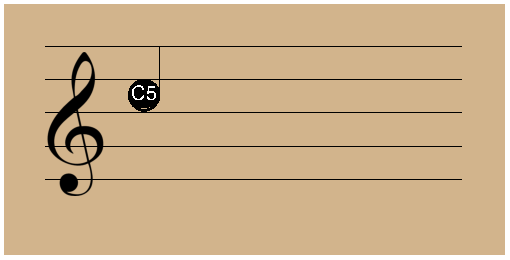
\includegraphics[trim=2.4000000000000004 2.4000000000000004 2.4000000000000004 2.4000000000000004]{pict.pdf}}}\end{SingleColumn}\end{RktBlk}\end{SCodeFlow}

\noindent This is a note called \Scribtexttt{C5}, or, C in the fifth octave.  It is sung by the soprano voice, for four
beats.

To play this note from the computer, we will convert it into a frequency.  A frequency will
be represented by the \RktSym{\badlink{\RktValLink{tone}}}\RktMeta{} object.  To turn notes into tones, we will use
a straightforward rewriter called \RktSym{\badlink{\RktValLink{note{-}{\Stttextmore}tone}}}\RktMeta{}. Tonart rewriters are not
composed into the context like objects; instead, they transform the context by
adding, deleting, and modifying existing objects.  Forms such as
\RktSym{\badlink{\RktValLink{define{-}art}}}\RktMeta{}, \RktSym{\badlink{\RktValLink{realize}}}\RktMeta{}, and \RktSym{\badlink{\RktValLink{@}}}\RktMeta{} evaluate their subforms from
top to bottom, applying rewriters only to the objects denoted above them.
\hspace*{\fill}\\


\noindent 

\noindent \begin{bigtabular}{@{\bigtableleftpad}l@{}l@{}l@{}l@{}}
\hbox{\mbox{\hphantom{\Scribtexttt{x}}}} &
\hbox{\textrm{$\langle$\textit{object}$\rangle$}} &
\hbox{\Scribtexttt{\mbox{\hphantom{\Scribtexttt{x}}}{\hbox{\texttt{:}}}{\hbox{\texttt{:}}}=\mbox{\hphantom{\Scribtexttt{x}}}}} &
\hbox{\RktInBG{\RktIn{{\hbox{\texttt{.}}}{\hbox{\texttt{.}}}{\hbox{\texttt{.}}}}}} \\
\hbox{\mbox{\hphantom{\Scribtexttt{x}}}} &
\hbox{ } &
\hbox{\Scribtexttt{\mbox{\hphantom{\Scribtexttt{x}}}\mbox{\hphantom{\Scribtexttt{x}}}{\Stttextbar}\mbox{\hphantom{\Scribtexttt{x}}}\mbox{\hphantom{\Scribtexttt{x}}}}} &
\hbox{\RktInBG{\RktIn{(}}\mbox{\hphantom{\Scribtexttt{x}}}\RktSym{\badlink{\RktValLink{tone}}}\RktMeta{}\mbox{\hphantom{\Scribtexttt{x}}}\textrm{$\langle$\textit{frequency}$\rangle$}\mbox{\hphantom{\Scribtexttt{x}}}\RktInBG{\RktIn{)}}} \\
\hbox{\mbox{\hphantom{\Scribtexttt{x}}}} &
\hbox{\textrm{$\langle$\textit{rewriter}$\rangle$}} &
\hbox{\Scribtexttt{\mbox{\hphantom{\Scribtexttt{x}}}{\hbox{\texttt{:}}}{\hbox{\texttt{:}}}=\mbox{\hphantom{\Scribtexttt{x}}}}} &
\hbox{\RktInBG{\RktIn{(}}\mbox{\hphantom{\Scribtexttt{x}}}\RktSym{\badlink{\RktValLink{note{-}{\Stttextmore}tone}}}\RktMeta{}\mbox{\hphantom{\Scribtexttt{x}}}\RktInBG{\RktIn{)}}} \\
\hbox{\mbox{\hphantom{\Scribtexttt{x}}}} &
\hbox{\textrm{$\langle$\textit{realizer}$\rangle$}} &
\hbox{\Scribtexttt{\mbox{\hphantom{\Scribtexttt{x}}}{\hbox{\texttt{:}}}{\hbox{\texttt{:}}}=\mbox{\hphantom{\Scribtexttt{x}}}}} &
\hbox{\RktInBG{\RktIn{{\hbox{\texttt{.}}}{\hbox{\texttt{.}}}{\hbox{\texttt{.}}}}}} \\
\hbox{\mbox{\hphantom{\Scribtexttt{x}}}} &
\hbox{ } &
\hbox{\Scribtexttt{\mbox{\hphantom{\Scribtexttt{x}}}\mbox{\hphantom{\Scribtexttt{x}}}{\Stttextbar}\mbox{\hphantom{\Scribtexttt{x}}}\mbox{\hphantom{\Scribtexttt{x}}}}} &
\hbox{\RktInBG{\RktIn{(}}\mbox{\hphantom{\Scribtexttt{x}}}\RktSym{sound{-}realizer}\RktMeta{}\mbox{\hphantom{\Scribtexttt{x}}}\RktInBG{\RktIn{)}}}\end{bigtabular}

\noindent \begin{SCentered}{---}{---}\end{SCentered}

\begin{SCodeFlow}\begin{RktBlk}\begin{SingleColumn}\RktPn{(}\RktSym{\badlink{\RktValLink{realize}}}\RktMeta{}\mbox{\hphantom{\Scribtexttt{x}}}\RktMeta{}\RktPn{(}\RktSym{sound{-}realizer}\RktPn{)}\RktMeta{}

\RktMeta{}\mbox{\hphantom{\Scribtexttt{xx}}}\RktMeta{}\RktPn{(}\RktSym{\badlink{\RktValLink{@}}}\RktMeta{}\mbox{\hphantom{\Scribtexttt{x}}}\RktMeta{}\RktPn{[}\RktPn{(}\RktSym{\badlink{\RktValLink{interval}}}\RktMeta{}\mbox{\hphantom{\Scribtexttt{x}}}\RktMeta{}\RktPn{[}\RktVal{0}\RktMeta{}\mbox{\hphantom{\Scribtexttt{x}}}\RktMeta{}\RktVal{4}\RktPn{]}\RktPn{)}\RktMeta{}\mbox{\hphantom{\Scribtexttt{x}}}\RktMeta{}\RktPn{(}\RktSym{\badlink{\RktValLink{voice}}}\RktMeta{}\mbox{\hphantom{\Scribtexttt{x}}}\RktMeta{}\RktSym{soprano}\RktPn{)}\RktPn{]}\RktMeta{}

\RktMeta{}\mbox{\hphantom{\Scribtexttt{xxxx}}}\RktMeta{}\RktPn{(}\RktSym{\badlink{\RktValLink{note}}}\RktMeta{}\mbox{\hphantom{\Scribtexttt{x}}}\RktMeta{}\RktSym{c}\RktMeta{}\mbox{\hphantom{\Scribtexttt{x}}}\RktMeta{}\RktVal{0}\RktMeta{}\mbox{\hphantom{\Scribtexttt{x}}}\RktMeta{}\RktVal{5}\RktPn{)}\RktPn{)}\RktMeta{}

\RktMeta{}\mbox{\hphantom{\Scribtexttt{xx}}}\RktMeta{}\RktPn{(}\RktSym{\badlink{\RktValLink{note{-}{\Stttextmore}tone}}}\RktPn{)}\RktPn{)}\RktMeta{}\end{SingleColumn}\end{RktBlk}\end{SCodeFlow}

\noindent Now we will add a harmony to this note.  We will express the harmony as a chord.
\hspace*{\fill}\\


\noindent 

\noindent \begin{bigtabular}{@{\bigtableleftpad}l@{}l@{}l@{}l@{}}
\hbox{\mbox{\hphantom{\Scribtexttt{x}}}} &
\hbox{\textrm{$\langle$\textit{object}$\rangle$}} &
\hbox{\Scribtexttt{\mbox{\hphantom{\Scribtexttt{x}}}{\hbox{\texttt{:}}}{\hbox{\texttt{:}}}=\mbox{\hphantom{\Scribtexttt{x}}}}} &
\hbox{\RktInBG{\RktIn{{\hbox{\texttt{.}}}{\hbox{\texttt{.}}}{\hbox{\texttt{.}}}}}} \\
\hbox{\mbox{\hphantom{\Scribtexttt{x}}}} &
\hbox{ } &
\hbox{\Scribtexttt{\mbox{\hphantom{\Scribtexttt{x}}}\mbox{\hphantom{\Scribtexttt{x}}}{\Stttextbar}\mbox{\hphantom{\Scribtexttt{x}}}\mbox{\hphantom{\Scribtexttt{x}}}}} &
\begin{tabular}[t]{@{}l@{}}
\hbox{\RktInBG{\RktIn{(}}\mbox{\hphantom{\Scribtexttt{x}}}\RktSym{\badlink{\RktValLink{chord}}}\RktMeta{}\mbox{\hphantom{\Scribtexttt{x}}}\textrm{$\langle$\textit{pitch}$\rangle$}\mbox{\hphantom{\Scribtexttt{x}}}\textrm{$\langle$\textit{accidental}$\rangle$}} \\
\hbox{\mbox{\hphantom{\Scribtexttt{x}}}\mbox{\hphantom{\Scribtexttt{x}}}\RktInBG{\RktIn{(}}\mbox{\hphantom{\Scribtexttt{x}}}\textrm{$\langle$\textit{quality}$\rangle$}\mbox{\hphantom{\Scribtexttt{x}}}\RktInBG{\RktIn{)}}\mbox{\hphantom{\Scribtexttt{x}}}\RktInBG{\RktIn{)}}}\end{tabular} \\
\hbox{\mbox{\hphantom{\Scribtexttt{x}}}} &
\hbox{\textrm{$\langle$\textit{rewriter}$\rangle$}} &
\hbox{\Scribtexttt{\mbox{\hphantom{\Scribtexttt{x}}}{\hbox{\texttt{:}}}{\hbox{\texttt{:}}}=\mbox{\hphantom{\Scribtexttt{x}}}}} &
\hbox{\RktInBG{\RktIn{{\hbox{\texttt{.}}}{\hbox{\texttt{.}}}{\hbox{\texttt{.}}}}}} \\
\hbox{\mbox{\hphantom{\Scribtexttt{x}}}} &
\hbox{ } &
\hbox{\Scribtexttt{\mbox{\hphantom{\Scribtexttt{x}}}\mbox{\hphantom{\Scribtexttt{x}}}{\Stttextbar}\mbox{\hphantom{\Scribtexttt{x}}}\mbox{\hphantom{\Scribtexttt{x}}}}} &
\hbox{\RktInBG{\RktIn{(}}\mbox{\hphantom{\Scribtexttt{x}}}\RktSym{chord{-}{\Stttextmore}notes}\RktMeta{}\mbox{\hphantom{\Scribtexttt{x}}}\textrm{$\langle$\textit{octave}$\rangle$}\mbox{\hphantom{\Scribtexttt{x}}}\RktInBG{\RktIn{)}}}\end{bigtabular}

\noindent \begin{SCentered}{---}{---}\end{SCentered}

\noindent For this demo, \RktSym{chord{-}{\Stttextmore}notes}\RktMeta{} simply writes in the first three
possible notes for each chord within its bounds, creating so{-}called {`}snowman{'} triads.  The number
specifies which octave the chords will start in.


\begin{SCodeFlow}\begin{RktBlk}\begin{SingleColumn}\begin{RktBlk}\begin{SingleColumn}\RktPn{(}\RktSym{\badlink{\RktValLink{realize}}}\mbox{\hphantom{\Scribtexttt{x}}}\RktPn{(}\RktSym{\badlink{\RktValLink{staff{-}realizer}}}\RktPn{)}

\mbox{\hphantom{\Scribtexttt{xx}}}\RktPn{(}\RktSym{\badlink{\RktValLink{@}}}\mbox{\hphantom{\Scribtexttt{x}}}\RktPn{[}\RktPn{(}\RktSym{\badlink{\RktValLink{interval}}}\mbox{\hphantom{\Scribtexttt{x}}}\RktPn{[}\RktVal{0}\mbox{\hphantom{\Scribtexttt{x}}}\RktVal{4}\RktPn{]}\RktPn{)}\mbox{\hphantom{\Scribtexttt{x}}}\RktPn{(}\RktSym{\badlink{\RktValLink{voice}}}\mbox{\hphantom{\Scribtexttt{x}}}\RktSym{accomp}\RktPn{)}\RktPn{]}

\mbox{\hphantom{\Scribtexttt{xxxx}}}\RktPn{(}\RktSym{\badlink{\RktValLink{chord}}}\mbox{\hphantom{\Scribtexttt{x}}}\RktSym{c}\mbox{\hphantom{\Scribtexttt{x}}}\RktVal{0}\mbox{\hphantom{\Scribtexttt{x}}}\RktPn{[}\RktSym{M}\RktPn{]}\RktPn{)}

\mbox{\hphantom{\Scribtexttt{xxxx}}}\RktPn{(}\RktSym{chord{-}{\Stttextmore}notes}\mbox{\hphantom{\Scribtexttt{x}}}\RktVal{3}\RktPn{)}\RktPn{)}\RktPn{)}\end{SingleColumn}\end{RktBlk}

\raisebox{-0.19999999999998863bp}{\makebox[240.0bp][l]{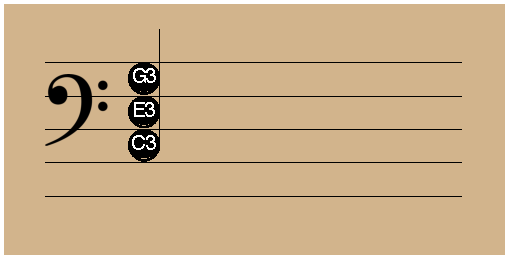
\includegraphics[trim=2.4000000000000004 2.4000000000000004 2.4000000000000004 2.4000000000000004]{pict_2.pdf}}}\end{SingleColumn}\end{RktBlk}\end{SCodeFlow}

We have not yet discussed putting objects one after another in time.  We could
of course use consecutive intervals.  However, this gets unwieldy.  We are
instead going to establish a concept of a \emph{sequence} of notes.
\hspace*{\fill}\\


\noindent 

\noindent \begin{bigtabular}{@{\bigtableleftpad}l@{}l@{}l@{}l@{}}
\hbox{\mbox{\hphantom{\Scribtexttt{x}}}} &
\hbox{\textrm{$\langle$\textit{context}$\rangle$}} &
\hbox{\Scribtexttt{\mbox{\hphantom{\Scribtexttt{x}}}{\hbox{\texttt{:}}}{\hbox{\texttt{:}}}=\mbox{\hphantom{\Scribtexttt{x}}}}} &
\hbox{\RktInBG{\RktIn{{\hbox{\texttt{.}}}{\hbox{\texttt{.}}}{\hbox{\texttt{.}}}}}} \\
\hbox{\mbox{\hphantom{\Scribtexttt{x}}}} &
\hbox{ } &
\hbox{\Scribtexttt{\mbox{\hphantom{\Scribtexttt{x}}}\mbox{\hphantom{\Scribtexttt{x}}}{\Stttextbar}\mbox{\hphantom{\Scribtexttt{x}}}\mbox{\hphantom{\Scribtexttt{x}}}}} &
\hbox{\RktInBG{\RktIn{(}}\mbox{\hphantom{\Scribtexttt{x}}}\RktSym{\badlink{\RktValLink{seq}}}\RktMeta{}\mbox{\hphantom{\Scribtexttt{x}}}\textrm{$\langle$\textit{form}$\rangle$}\textrm{*}\mbox{\hphantom{\Scribtexttt{x}}}\RktInBG{\RktIn{)}}} \\
\hbox{\mbox{\hphantom{\Scribtexttt{x}}}} &
\hbox{\textrm{$\langle$\textit{coordinate}$\rangle$}} &
\hbox{\Scribtexttt{\mbox{\hphantom{\Scribtexttt{x}}}{\hbox{\texttt{:}}}{\hbox{\texttt{:}}}=\mbox{\hphantom{\Scribtexttt{x}}}}} &
\hbox{\RktInBG{\RktIn{{\hbox{\texttt{.}}}{\hbox{\texttt{.}}}{\hbox{\texttt{.}}}}}} \\
\hbox{\mbox{\hphantom{\Scribtexttt{x}}}} &
\hbox{ } &
\hbox{\Scribtexttt{\mbox{\hphantom{\Scribtexttt{x}}}\mbox{\hphantom{\Scribtexttt{x}}}{\Stttextbar}\mbox{\hphantom{\Scribtexttt{x}}}\mbox{\hphantom{\Scribtexttt{x}}}}} &
\hbox{\RktInBG{\RktIn{(}}\mbox{\hphantom{\Scribtexttt{x}}}\RktSym{\badlink{\RktValLink{index}}}\RktMeta{}\mbox{\hphantom{\Scribtexttt{x}}}\textrm{$\langle$\textit{number}$\rangle$}\textrm{*}\mbox{\hphantom{\Scribtexttt{x}}}\RktInBG{\RktIn{)}}}\end{bigtabular}

\noindent \hspace*{\fill}\\
We define a new context.  This context is called \RktSym{\badlink{\RktValLink{seq}}}\RktMeta{} and has one coordinate, \RktSym{\badlink{\RktValLink{index}}}\RktMeta{},
representing the position of an object in the context.  \RktSym{\badlink{\RktValLink{seq}}}\RktMeta{} contexts can be embedded in music
contexts, allowing us to express an ordered sequence directly in a score, without
giving specific lengths to the notes or other objects it contains.

Next, we define syntax for rhythms, which are, for our purposes, a series of consecutive durations.
\hspace*{\fill}\\


\noindent 

\noindent \begin{bigtabular}{@{\bigtableleftpad}l@{}l@{}l@{}l@{}}
\hbox{\mbox{\hphantom{\Scribtexttt{x}}}} &
\hbox{\textrm{$\langle$\textit{object}$\rangle$}} &
\hbox{\Scribtexttt{\mbox{\hphantom{\Scribtexttt{x}}}{\hbox{\texttt{:}}}{\hbox{\texttt{:}}}=\mbox{\hphantom{\Scribtexttt{x}}}}} &
\hbox{\RktInBG{\RktIn{{\hbox{\texttt{.}}}{\hbox{\texttt{.}}}{\hbox{\texttt{.}}}}}} \\
\hbox{\mbox{\hphantom{\Scribtexttt{x}}}} &
\hbox{ } &
\hbox{\Scribtexttt{\mbox{\hphantom{\Scribtexttt{x}}}\mbox{\hphantom{\Scribtexttt{x}}}{\Stttextbar}\mbox{\hphantom{\Scribtexttt{x}}}\mbox{\hphantom{\Scribtexttt{x}}}}} &
\hbox{\RktInBG{\RktIn{(}}\mbox{\hphantom{\Scribtexttt{x}}}\RktSym{\badlink{\RktValLink{rhythm}}}\RktMeta{}\mbox{\hphantom{\Scribtexttt{x}}}\textrm{$\langle$\textit{number}$\rangle$}\textrm{*}\mbox{\hphantom{\Scribtexttt{x}}}\RktInBG{\RktIn{)}}} \\
\hbox{\mbox{\hphantom{\Scribtexttt{x}}}} &
\hbox{\textrm{$\langle$\textit{rewriter}$\rangle$}} &
\hbox{\Scribtexttt{\mbox{\hphantom{\Scribtexttt{x}}}{\hbox{\texttt{:}}}{\hbox{\texttt{:}}}=\mbox{\hphantom{\Scribtexttt{x}}}}} &
\hbox{\RktInBG{\RktIn{{\hbox{\texttt{.}}}{\hbox{\texttt{.}}}{\hbox{\texttt{.}}}}}} \\
\hbox{\mbox{\hphantom{\Scribtexttt{x}}}} &
\hbox{ } &
\hbox{\Scribtexttt{\mbox{\hphantom{\Scribtexttt{x}}}\mbox{\hphantom{\Scribtexttt{x}}}{\Stttextbar}\mbox{\hphantom{\Scribtexttt{x}}}\mbox{\hphantom{\Scribtexttt{x}}}}} &
\hbox{\RktInBG{\RktIn{(}}\mbox{\hphantom{\Scribtexttt{x}}}\RktSym{\badlink{\RktValLink{apply{-}rhythm}}}\RktMeta{}\mbox{\hphantom{\Scribtexttt{x}}}\RktInBG{\RktIn{)}}}\end{bigtabular}

\noindent \hspace*{\fill}\\
Now we can do something more complex with the soprano.
\hspace*{\fill}\\
Note: Instead of writing,


\begin{SCodeFlow}\begin{RktBlk}\begin{SingleColumn}\RktPn{(}\RktSym{\badlink{\RktValLink{seq}}}\RktMeta{}

\RktMeta{}\mbox{\hphantom{\Scribtexttt{xx}}}\RktMeta{}\RktPn{(}\RktSym{\badlink{\RktValLink{@}}}\RktMeta{}\mbox{\hphantom{\Scribtexttt{x}}}\RktMeta{}\RktPn{[}\RktPn{(}\RktSym{\badlink{\RktValLink{index}}}\RktMeta{}\mbox{\hphantom{\Scribtexttt{x}}}\RktMeta{}\RktVal{0}\RktPn{)}\RktPn{]}\RktMeta{}\mbox{\hphantom{\Scribtexttt{x}}}\RktMeta{}\RktPn{(}\RktSym{\badlink{\RktValLink{note}}}\RktMeta{}\mbox{\hphantom{\Scribtexttt{x}}}\RktMeta{}\RktSym{a}\RktMeta{}\mbox{\hphantom{\Scribtexttt{x}}}\RktMeta{}\RktVal{0}\RktMeta{}\mbox{\hphantom{\Scribtexttt{x}}}\RktMeta{}\RktVal{3}\RktPn{)}\RktPn{)}\RktMeta{}

\RktMeta{}\mbox{\hphantom{\Scribtexttt{xx}}}\RktMeta{}\RktPn{(}\RktSym{\badlink{\RktValLink{@}}}\RktMeta{}\mbox{\hphantom{\Scribtexttt{x}}}\RktMeta{}\RktPn{[}\RktPn{(}\RktSym{\badlink{\RktValLink{index}}}\RktMeta{}\mbox{\hphantom{\Scribtexttt{x}}}\RktMeta{}\RktVal{1}\RktPn{)}\RktPn{]}\RktMeta{}\mbox{\hphantom{\Scribtexttt{x}}}\RktMeta{}\RktPn{(}\RktSym{\badlink{\RktValLink{note}}}\RktMeta{}\mbox{\hphantom{\Scribtexttt{x}}}\RktMeta{}\RktSym{b}\RktMeta{}\mbox{\hphantom{\Scribtexttt{x}}}\RktMeta{}\RktVal{0}\RktMeta{}\mbox{\hphantom{\Scribtexttt{x}}}\RktMeta{}\RktVal{3}\RktPn{)}\RktPn{)}\RktMeta{}

\RktMeta{}\mbox{\hphantom{\Scribtexttt{xx}}}\RktMeta{}\RktSym{{\hbox{\texttt{.}}}{\hbox{\texttt{.}}}{\hbox{\texttt{.}}}}\RktPn{)}\RktMeta{}\end{SingleColumn}\end{RktBlk}\end{SCodeFlow}

\noindent I will write \RktPn{(}\RktSym{\badlink{\RktValLink{seq}}}\RktMeta{}\mbox{\hphantom{\Scribtexttt{x}}}\RktMeta{}\RktPn{(}\RktSym{\badlink{\RktValLink{notes}}}\RktMeta{}\mbox{\hphantom{\Scribtexttt{x}}}\RktMeta{}\RktPn{[}\RktSym{a}\RktMeta{}\mbox{\hphantom{\Scribtexttt{x}}}\RktMeta{}\RktVal{0}\RktMeta{}\mbox{\hphantom{\Scribtexttt{x}}}\RktMeta{}\RktVal{3}\RktPn{]}\RktMeta{}\mbox{\hphantom{\Scribtexttt{x}}}\RktMeta{}\RktPn{[}\RktSym{b}\RktMeta{}\mbox{\hphantom{\Scribtexttt{x}}}\RktMeta{}\RktVal{0}\RktMeta{}\mbox{\hphantom{\Scribtexttt{x}}}\RktMeta{}\RktVal{3}\RktPn{]}\RktMeta{}\mbox{\hphantom{\Scribtexttt{x}}}\RktMeta{}\RktSym{{\hbox{\texttt{.}}}{\hbox{\texttt{.}}}{\hbox{\texttt{.}}}}\RktPn{)}\RktPn{)}\RktMeta{}.
\hspace*{\fill}\\
Below, a melody is bound.

\begin{SCodeFlow}\begin{RktBlk}\begin{SingleColumn}\begin{RktBlk}\begin{SingleColumn}\RktPn{(}\RktSym{\badlink{\RktValLink{define{-}art}}}\mbox{\hphantom{\Scribtexttt{x}}}\RktSym{melody}

\mbox{\hphantom{\Scribtexttt{xx}}}\RktPn{(}\RktSym{\badlink{\RktValLink{seq}}}\mbox{\hphantom{\Scribtexttt{x}}}\RktPn{(}\RktSym{\badlink{\RktValLink{notes}}}\mbox{\hphantom{\Scribtexttt{x}}}\RktPn{[}\RktSym{c}\mbox{\hphantom{\Scribtexttt{x}}}\RktVal{0}\mbox{\hphantom{\Scribtexttt{x}}}\RktVal{5}\RktPn{]}\mbox{\hphantom{\Scribtexttt{x}}}\RktPn{[}\RktSym{b}\mbox{\hphantom{\Scribtexttt{x}}}\RktVal{\mbox{{-}1}}\mbox{\hphantom{\Scribtexttt{x}}}\RktVal{4}\RktPn{]}\mbox{\hphantom{\Scribtexttt{x}}}\RktPn{[}\RktSym{a}\mbox{\hphantom{\Scribtexttt{x}}}\RktVal{0}\mbox{\hphantom{\Scribtexttt{x}}}\RktVal{4}\RktPn{]}

\mbox{\hphantom{\Scribtexttt{xxxxxxxxxxxxxx}}}\RktPn{[}\RktSym{b}\mbox{\hphantom{\Scribtexttt{x}}}\RktVal{0}\mbox{\hphantom{\Scribtexttt{x}}}\RktVal{4}\RktPn{]}\mbox{\hphantom{\Scribtexttt{x}}}\RktPn{[}\RktSym{c}\mbox{\hphantom{\Scribtexttt{x}}}\RktVal{0}\mbox{\hphantom{\Scribtexttt{x}}}\RktVal{5}\RktPn{]}\RktPn{)}\RktPn{)}

\mbox{\hphantom{\Scribtexttt{xx}}}\RktPn{(}\RktSym{\badlink{\RktValLink{rhythm}}}\mbox{\hphantom{\Scribtexttt{x}}}\RktVal{3/2}\mbox{\hphantom{\Scribtexttt{x}}}\RktVal{1/2}\mbox{\hphantom{\Scribtexttt{x}}}\RktVal{1/2}\mbox{\hphantom{\Scribtexttt{x}}}\RktVal{3/2}\mbox{\hphantom{\Scribtexttt{x}}}\RktVal{2}\RktPn{)}\RktPn{)}\end{SingleColumn}\end{RktBlk}\end{SingleColumn}\end{RktBlk}\end{SCodeFlow}

Now, we supply a harmony, which the accompaniment will outline.

\begin{SCodeFlow}\begin{RktBlk}\begin{SingleColumn}\begin{RktBlk}\begin{SingleColumn}\RktPn{(}\RktSym{\badlink{\RktValLink{define{-}art}}}\mbox{\hphantom{\Scribtexttt{x}}}\RktSym{harmony}

\mbox{\hphantom{\Scribtexttt{xxxx}}}\RktPn{(}\RktSym{\badlink{\RktValLink{seq}}}\mbox{\hphantom{\Scribtexttt{x}}}\RktPn{(}\RktSym{\badlink{\RktValLink{chords}}}\mbox{\hphantom{\Scribtexttt{x}}}\RktPn{[}\RktSym{f}\mbox{\hphantom{\Scribtexttt{x}}}\RktVal{0}\mbox{\hphantom{\Scribtexttt{x}}}\RktSym{M}\RktPn{]}\mbox{\hphantom{\Scribtexttt{x}}}\RktPn{[}\RktSym{c}\mbox{\hphantom{\Scribtexttt{x}}}\RktVal{0}\mbox{\hphantom{\Scribtexttt{x}}}\RktSym{M}\RktPn{]}\mbox{\hphantom{\Scribtexttt{x}}}\RktPn{[}\RktSym{f}\mbox{\hphantom{\Scribtexttt{x}}}\RktVal{0}\mbox{\hphantom{\Scribtexttt{x}}}\RktSym{M}\RktPn{]}

\mbox{\hphantom{\Scribtexttt{xxxxxxxxxxxxxxxxx}}}\RktPn{[}\RktSym{g}\mbox{\hphantom{\Scribtexttt{x}}}\RktVal{0}\mbox{\hphantom{\Scribtexttt{x}}}\RktSym{M}\RktPn{]}\mbox{\hphantom{\Scribtexttt{x}}}\RktPn{[}\RktSym{c}\mbox{\hphantom{\Scribtexttt{x}}}\RktVal{0}\mbox{\hphantom{\Scribtexttt{x}}}\RktSym{M}\RktPn{]}\RktPn{)}\RktPn{)}

\mbox{\hphantom{\Scribtexttt{xxxx}}}\RktPn{(}\RktSym{\badlink{\RktValLink{rhythm}}}\mbox{\hphantom{\Scribtexttt{x}}}\RktVal{1}\mbox{\hphantom{\Scribtexttt{x}}}\RktVal{1}\mbox{\hphantom{\Scribtexttt{x}}}\RktVal{1}\mbox{\hphantom{\Scribtexttt{x}}}\RktVal{1}\mbox{\hphantom{\Scribtexttt{x}}}\RktVal{2}\RktPn{)}\RktPn{)}\end{SingleColumn}\end{RktBlk}\end{SingleColumn}\end{RktBlk}\end{SCodeFlow}

\noindent We compose them together, and rewrite the piece into notes.


\begin{SCodeFlow}\begin{RktBlk}\begin{SingleColumn}\begin{RktBlk}\begin{SingleColumn}\RktPn{(}\RktSym{\badlink{\RktValLink{define{-}art}}}\mbox{\hphantom{\Scribtexttt{x}}}\RktSym{song{-}notes}

\mbox{\hphantom{\Scribtexttt{xx}}}\RktPn{(}\RktSym{\badlink{\RktValLink{voice@}}}\mbox{\hphantom{\Scribtexttt{x}}}\RktPn{(}\RktSym{soprano}\RktPn{)}\mbox{\hphantom{\Scribtexttt{x}}}\RktSym{melody}\RktPn{)}

\mbox{\hphantom{\Scribtexttt{xx}}}\RktPn{(}\RktSym{\badlink{\RktValLink{voice@}}}\mbox{\hphantom{\Scribtexttt{x}}}\RktPn{(}\RktSym{accomp}\RktPn{)}\mbox{\hphantom{\Scribtexttt{x}}}\RktSym{harmony}\RktPn{)}

\mbox{\hphantom{\Scribtexttt{xx}}}\RktPn{(}\RktSym{\badlink{\RktValLink{apply{-}rhythm}}}\RktPn{)}\mbox{\hphantom{\Scribtexttt{x}}}\RktPn{(}\RktSym{chord{-}{\Stttextmore}notes}\mbox{\hphantom{\Scribtexttt{x}}}\RktVal{3}\RktPn{)}\RktPn{)}\end{SingleColumn}\end{RktBlk}\end{SingleColumn}\end{RktBlk}\end{SCodeFlow}

Note that the use of \RktSym{\badlink{\RktValLink{apply{-}rhythm}}}\RktMeta{} above applies both the rhythm of the
melody, and the harmonic rhythm of the harmony.
\hspace*{\fill}\\
To see it visualized:


\begin{SCodeFlow}\begin{RktBlk}\begin{SingleColumn}\begin{RktBlk}\begin{SingleColumn}\RktPn{(}\RktSym{\badlink{\RktValLink{realize}}}\mbox{\hphantom{\Scribtexttt{x}}}\RktPn{(}\RktSym{\badlink{\RktValLink{staff{-}realizer}}}\RktPn{)}

\mbox{\hphantom{\Scribtexttt{xx}}}\RktSym{song{-}notes}\RktPn{)}\end{SingleColumn}\end{RktBlk}

\raisebox{-0.19999999999998863bp}{\makebox[240.0bp][l]{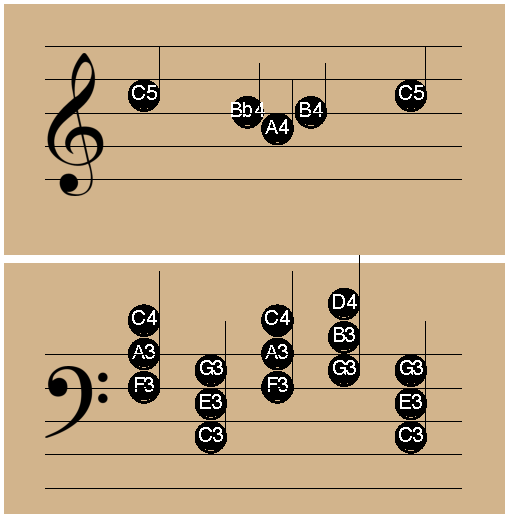
\includegraphics[trim=2.4000000000000004 2.4000000000000004 2.4000000000000004 2.4000000000000004]{pict_3.pdf}}}\end{SingleColumn}\end{RktBlk}\end{SCodeFlow}

\noindent To hear it:


\begin{SCodeFlow}\begin{RktBlk}\begin{SingleColumn}\RktPn{(}\RktSym{\badlink{\RktValLink{realize}}}\RktMeta{}\mbox{\hphantom{\Scribtexttt{x}}}\RktMeta{}\RktPn{(}\RktSym{sound{-}realizer}\RktPn{)}\RktMeta{}

\RktMeta{}\mbox{\hphantom{\Scribtexttt{xx}}}\RktMeta{}\RktSym{song{-}notes}\RktMeta{}\mbox{\hphantom{\Scribtexttt{x}}}\RktMeta{}\RktPn{(}\RktSym{\badlink{\RktValLink{note{-}{\Stttextmore}tone}}}\RktPn{)}\RktPn{)}\RktMeta{}\end{SingleColumn}\end{RktBlk}\end{SCodeFlow}

\Ssubsection{Finale}{Finale}\label{t:x28part_x22Finalex22x29}

To finish off, we will try adding a more obscure object to our composition.
\hspace*{\fill}\\


\noindent 

\noindent \begin{bigtabular}{@{\bigtableleftpad}l@{}l@{}l@{}l@{}}
\hbox{\mbox{\hphantom{\Scribtexttt{x}}}} &
\hbox{\textrm{$\langle$\textit{object}$\rangle$}} &
\hbox{\Scribtexttt{\mbox{\hphantom{\Scribtexttt{x}}}{\hbox{\texttt{:}}}{\hbox{\texttt{:}}}=\mbox{\hphantom{\Scribtexttt{x}}}}} &
\hbox{\RktInBG{\RktIn{{\hbox{\texttt{.}}}{\hbox{\texttt{.}}}{\hbox{\texttt{.}}}}}} \\
\hbox{\mbox{\hphantom{\Scribtexttt{x}}}} &
\hbox{ } &
\hbox{\Scribtexttt{\mbox{\hphantom{\Scribtexttt{x}}}\mbox{\hphantom{\Scribtexttt{x}}}{\Stttextbar}\mbox{\hphantom{\Scribtexttt{x}}}\mbox{\hphantom{\Scribtexttt{x}}}}} &
\hbox{\RktInBG{\RktIn{(}}\mbox{\hphantom{\Scribtexttt{x}}}\RktSym{\badlink{\RktValLink{function}}}\RktMeta{}\mbox{\hphantom{\Scribtexttt{x}}}\RktInBG{\RktIn{(}}\mbox{\hphantom{\Scribtexttt{x}}}\textrm{$\langle$\textit{id}$\rangle$}\mbox{\hphantom{\Scribtexttt{x}}}\RktInBG{\RktIn{)}}\mbox{\hphantom{\Scribtexttt{x}}}\textrm{$\langle$\textit{expr}$\rangle$}\mbox{\hphantom{\Scribtexttt{x}}}\RktInBG{\RktIn{)}}} \\
\hbox{\mbox{\hphantom{\Scribtexttt{x}}}} &
\hbox{\textrm{$\langle$\textit{rewriter}$\rangle$}} &
\hbox{\Scribtexttt{\mbox{\hphantom{\Scribtexttt{x}}}{\hbox{\texttt{:}}}{\hbox{\texttt{:}}}=\mbox{\hphantom{\Scribtexttt{x}}}}} &
\hbox{\RktInBG{\RktIn{{\hbox{\texttt{.}}}{\hbox{\texttt{.}}}{\hbox{\texttt{.}}}}}} \\
\hbox{\mbox{\hphantom{\Scribtexttt{x}}}} &
\hbox{ } &
\hbox{\Scribtexttt{\mbox{\hphantom{\Scribtexttt{x}}}\mbox{\hphantom{\Scribtexttt{x}}}{\Stttextbar}\mbox{\hphantom{\Scribtexttt{x}}}\mbox{\hphantom{\Scribtexttt{x}}}}} &
\begin{tabular}[t]{@{}l@{}}
\hbox{\RktInBG{\RktIn{(}}\mbox{\hphantom{\Scribtexttt{x}}}\RktSym{function{-}{\Stttextmore}notes}\RktMeta{}} \\
\hbox{\mbox{\hphantom{\Scribtexttt{x}}}\mbox{\hphantom{\Scribtexttt{x}}}\RktInBG{\RktIn{(}}\mbox{\hphantom{\Scribtexttt{x}}}\textrm{$\langle$\textit{number}$\rangle$}\mbox{\hphantom{\Scribtexttt{x}}}\textrm{$\langle$\textit{number}$\rangle$}\mbox{\hphantom{\Scribtexttt{x}}}\RktInBG{\RktIn{)}}} \\
\hbox{\mbox{\hphantom{\Scribtexttt{x}}}\mbox{\hphantom{\Scribtexttt{x}}}\RktInBG{\RktIn{(}}\mbox{\hphantom{\Scribtexttt{x}}}\textrm{$\langle$\textit{note}$\rangle$}\mbox{\hphantom{\Scribtexttt{x}}}\textrm{$\langle$\textit{note}$\rangle$}\mbox{\hphantom{\Scribtexttt{x}}}\RktInBG{\RktIn{)}}\mbox{\hphantom{\Scribtexttt{x}}}\RktInBG{\RktIn{)}}}\end{tabular}\end{bigtabular}

\noindent \hspace*{\fill}\\
\RktSym{\badlink{\RktValLink{function}}}\RktMeta{} is a mathematical function.

\RktSym{function{-}{\Stttextmore}notes}\RktMeta{} applies to functions, and it creates a melody that fits within the surrounding
harmony and matches the contour of the function.

Here is the finished work. I will use \RktPn{(}\RktSym{\badlink{\RktValLink{uniform{-}rhythm}}}\RktMeta{}\mbox{\hphantom{\Scribtexttt{x}}}\RktMeta{}\RktVal{1/4}\RktPn{)}\RktMeta{} as a shorthand for
\RktPn{(}\RktSym{\badlink{\RktValLink{rhythm}}}\RktMeta{}\mbox{\hphantom{\Scribtexttt{x}}}\RktMeta{}\RktVal{1/4}\RktMeta{}\mbox{\hphantom{\Scribtexttt{x}}}\RktMeta{}\RktVal{1/4}\RktMeta{}\mbox{\hphantom{\Scribtexttt{x}}}\RktMeta{}\RktVal{1/4}\RktMeta{}\mbox{\hphantom{\Scribtexttt{x}}}\RktMeta{}\RktSym{{\hbox{\texttt{.}}}{\hbox{\texttt{.}}}{\hbox{\texttt{.}}}}\RktPn{)}\RktMeta{}.  The function is \texMathInline{sin(x)} over \texMathInline{(-\pi,\pi)}.


\begin{SCodeFlow}\begin{RktBlk}\begin{SingleColumn}\begin{RktBlk}\begin{SingleColumn}\RktPn{(}\RktSym{\badlink{\RktValLink{realize}}}\mbox{\hphantom{\Scribtexttt{x}}}\RktPn{(}\RktSym{\badlink{\RktValLink{staff{-}realizer}}}\RktPn{)}

\mbox{\hphantom{\Scribtexttt{xx}}}\RktSym{song{-}notes}

\mbox{\hphantom{\Scribtexttt{xx}}}\RktPn{(}\RktSym{\badlink{\RktValLink{@}}}\mbox{\hphantom{\Scribtexttt{x}}}\RktPn{[}\RktPn{(}\RktSym{\badlink{\RktValLink{voice}}}\mbox{\hphantom{\Scribtexttt{x}}}\RktSym{countermelody}\RktPn{)}\RktPn{]}

\mbox{\hphantom{\Scribtexttt{xxxx}}}\RktSym{harmony}\mbox{\hphantom{\Scribtexttt{x}}}\RktPn{(}\RktSym{\badlink{\RktValLink{apply{-}rhythm}}}\RktPn{)}

\mbox{\hphantom{\Scribtexttt{xxxx}}}\RktPn{(}\RktSym{\badlink{\RktValLink{@}}}\mbox{\hphantom{\Scribtexttt{x}}}\RktPn{[}\RktPn{(}\RktSym{\badlink{\RktValLink{interval}}}\mbox{\hphantom{\Scribtexttt{x}}}\RktPn{[}\RktVal{0}\mbox{\hphantom{\Scribtexttt{x}}}\RktVal{5}\RktPn{]}\RktPn{)}\RktPn{]}

\mbox{\hphantom{\Scribtexttt{xxxxxx}}}\RktPn{(}\RktSym{\badlink{\RktValLink{function}}}\mbox{\hphantom{\Scribtexttt{x}}}\RktPn{(}\RktSym{x}\RktPn{)}\mbox{\hphantom{\Scribtexttt{x}}}\RktPn{(}\RktSym{sin}\mbox{\hphantom{\Scribtexttt{x}}}\RktSym{x}\RktPn{)}\RktPn{)}

\mbox{\hphantom{\Scribtexttt{xxxxxx}}}\RktPn{(}\RktSym{\badlink{\RktValLink{uniform{-}rhythm}}}\mbox{\hphantom{\Scribtexttt{x}}}\RktVal{1/4}\RktPn{)}\RktPn{)}

\mbox{\hphantom{\Scribtexttt{xxxx}}}\RktPn{(}\RktSym{\badlink{\RktValLink{@}}}\mbox{\hphantom{\Scribtexttt{x}}}\RktPn{[}\RktPn{(}\RktSym{\badlink{\RktValLink{interval}}}\mbox{\hphantom{\Scribtexttt{x}}}\RktPn{[}\RktVal{5}\mbox{\hphantom{\Scribtexttt{x}}}\RktVal{6}\RktPn{]}\RktPn{)}\RktPn{]}\mbox{\hphantom{\Scribtexttt{x}}}\RktPn{(}\RktSym{\badlink{\RktValLink{note}}}\mbox{\hphantom{\Scribtexttt{x}}}\RktSym{e}\mbox{\hphantom{\Scribtexttt{x}}}\RktVal{0}\mbox{\hphantom{\Scribtexttt{x}}}\RktVal{4}\RktPn{)}\RktPn{)}

\mbox{\hphantom{\Scribtexttt{xxxx}}}\RktPn{(}\RktSym{function{-}{\Stttextmore}notes}\mbox{\hphantom{\Scribtexttt{x}}}\RktPn{[}\RktPn{(}\RktSym{\mbox{{-}}}\mbox{\hphantom{\Scribtexttt{x}}}\RktSym{pi}\RktPn{)}\mbox{\hphantom{\Scribtexttt{x}}}\RktSym{pi}\RktPn{]}\mbox{\hphantom{\Scribtexttt{x}}}\RktPn{[}\RktPn{(}\RktSym{a}\mbox{\hphantom{\Scribtexttt{x}}}\RktVal{3}\RktPn{)}\mbox{\hphantom{\Scribtexttt{x}}}\RktPn{(}\RktSym{a}\mbox{\hphantom{\Scribtexttt{x}}}\RktVal{4}\RktPn{)}\RktPn{]}\RktPn{)}\RktPn{)}\RktPn{)}\end{SingleColumn}\end{RktBlk}

\raisebox{-0.7999999999999545bp}{\makebox[240.0bp][l]{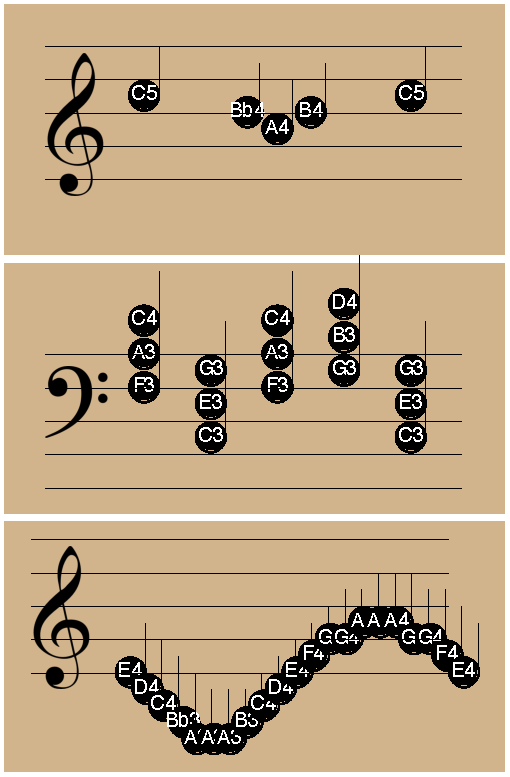
\includegraphics[trim=2.4000000000000004 2.4000000000000004 2.4000000000000004 2.4000000000000004]{pict_4.pdf}}}\end{SingleColumn}\end{RktBlk}\end{SCodeFlow}

\sectionNewpage

%%% -*-BibTeX-*-
%%% Do NOT edit. File created by BibTeX with style
%%% ACM-Reference-Format-Journals [18-Jan-2012].

\begin{thebibliography}{2}

%%% ====================================================================
%%% NOTE TO THE USER: you can override these defaults by providing
%%% customized versions of any of these macros before the \bibliography
%%% command.  Each of them MUST provide its own final punctuation,
%%% except for \shownote{}, \showDOI{}, and \showURL{}.  The latter two
%%% do not use final punctuation, in order to avoid confusing it with
%%% the Web address.
%%%
%%% To suppress output of a particular field, define its macro to expand
%%% to an empty string, or better, \unskip, like this:
%%%
%%% \newcommand{\showDOI}[1]{\unskip}   % LaTeX syntax
%%%
%%% \def \showDOI #1{\unskip}           % plain TeX syntax
%%%
%%% ====================================================================

\ifx \showCODEN    \undefined \def \showCODEN     #1{\unskip}     \fi
\ifx \showDOI      \undefined \def \showDOI       #1{#1}\fi
\ifx \showISBNx    \undefined \def \showISBNx     #1{\unskip}     \fi
\ifx \showISBNxiii \undefined \def \showISBNxiii  #1{\unskip}     \fi
\ifx \showISSN     \undefined \def \showISSN      #1{\unskip}     \fi
\ifx \showLCCN     \undefined \def \showLCCN      #1{\unskip}     \fi
\ifx \shownote     \undefined \def \shownote      #1{#1}          \fi
\ifx \showarticletitle \undefined \def \showarticletitle #1{#1}   \fi
\ifx \showURL      \undefined \def \showURL       {\relax}        \fi
% The following commands are used for tagged output and should be
% invisible to TeX
\providecommand\bibfield[2]{#2}
\providecommand\bibinfo[2]{#2}
\providecommand\natexlab[1]{#1}
\providecommand\showeprint[2][]{arXiv:#2}

\bibitem[Flatt(2002)]%
        {ywiw}
\bibfield{author}{\bibinfo{person}{Matthew Flatt}.}
  \bibinfo{year}{2002}\natexlab{}.
\newblock \showarticletitle{Composable and Compilable Macros: You Want it
  When?}. In \bibinfo{booktitle}{\emph{Proceedings of the ACM Intl. Conf.
  Functional Programming}}. \bibinfo{pages}{72--83}.
\newblock


\bibitem[Hudak(2014)]%
        {euterp}
\bibfield{author}{\bibinfo{person}{Paul Hudak}.}
  \bibinfo{year}{2014}\natexlab{}.
\newblock \bibinfo{title}{Euterpea}.
\newblock
\newblock
\urldef\tempurl%
\url{http://euterpea.com}
\showURL{%
\tempurl}


\end{thebibliography}


\postDoc
\end{document}
